% Template LaTeX document for CSSR4Africa Deliverables
% Adapted from documents prepared by EPFL for the RobotCub project
% and subsequently by the University of Skövde for the DREAM project
%
% DV 28/06/2023

\documentclass{CSSRforAfrica}

\usepackage[hidelinks,colorlinks=false]{hyperref}
\usepackage[titletoc,title]{appendix}
\usepackage{latexsym}
\usepackage{tabularx,colortbl}
\usepackage{verbatim} % for comments
\usepackage{makecell} % forrmatting tables.


\newcommand{\blank}{~\\}
\newcommand{\checkbox}{{~~~~~~~\leavevmode \put(-7,-1.5){  \huge $\Box$  }}}

\begin{document}
\input{epsf}

%%
%% SHOULD NOT NEED TO BE CHANGED BEFORE THIS POINT
%% ------------------------------------------------
%%

\deliverable{D3.1}               
\title{D3.1 System Architecture}  

\leadpartner{Carnegie Mellon University Africa}     
%%\partner{}                               

\revision{2.6}                         
\deliverabledate{31/01/2024}    
\submissiondate{24/01/2024}   
\revisiondate{11/06/2025}   
\disseminationlevel{PU}
\responsible{D. Vernon }            


%%
%% Create the titlepage
%%

\maketitle
 

\section*{Executive Summary}
%###############################
\label{executive_summary}
%%\addcontentsline{toc}{section}{Executive Summary}
 
This deliverable represents the outcome of Task 3.1.  It specifies the CSSR4Africa system architecture in detail, identifying the component subsystems, the modules (i.e., ROS nodes) comprising each subsystem, and the information exchanged between subsystems and modules. This includes a specification of the data that are input to each module, the data that are output from each module, and the data that are used to control the operation of the module, including the manner in which this data is made available or accessed: through ROS topics, services, or actions, or through input and configuration files.

Based on the ROS nodes identified in  Deliverables D2.2 and D2.3, Deliverable D3.1 provides the requirements for work package WP4 and WP5 on robot  sensing and action, complementing and augmenting the detailed specification already provided in the work plan, as well as providing the architecture for the integration of the ROS nodes in each subsystem into a complete operational robot control system. 

\newpage
 
 
%\graphicspath{{./figs/}}
\pagebreak
\tableofcontents
\newpage

\section{Introduction}
%###############################



This deliverable, D3.1 System Architecture Design,  provides a detailed specification of the architecture of the CSSR4Africa software system that controls the culturally sensitive social interaction between the Pepper robot and a human, i.e., a visitor in one of the two use case scenarios specified in Deliverable D2.1.   

It specifies the  architecture's component subsystems, the modules (i.e., ROS nodes) comprising each subsystem, and the information exchanged between each  module. This includes a specification of the data that are input to each module, the data that are output from each module, and the data that are used to control the operation of the module, including the manner in which this data is made available or accessed:  through ROS topics, services, or actions, or through input and configuration files.

Based on the ROS nodes identified in  Deliverables D2.2 and D2.3, Deliverable D3.1 provides the requirements for work package WP4 and WP5 on robot  sensing and action, complementing and augmenting the detailed specification already provided in the work plan, as well as providing the architecture for the integration of the ROS nodes in each subsystem into a complete operational robot control system. 

For each ROS node, the deliverable specifies the node configuration parameters that are read from the associated configuration file, the data that are read from the associated input file, the data that are written to an associated output file, the ROS topics to which the node subscribes for input,  the ROS topics to which the node publishes output, the services that will be advertized and served, and the services that will be invoked.

The dynamics of the interaction between the visitor and the robot, implemented with these  ROS nodes, will be specified in Deliverable D5.4.2 Robot Mission Language, and implemented in the {\small \verb+behaviorController+} node in Deliverable D5.4.3 Robot Mission Interpreter.

In the following, we provide a high-level overview of the system architecture, a specification of each constituent ROS node, and detailed architecture that includes the topics published by each node, the topics each node subscribes to, and the services advertised and served by each node.


\begin{figure}[tbh]
\begin{center}
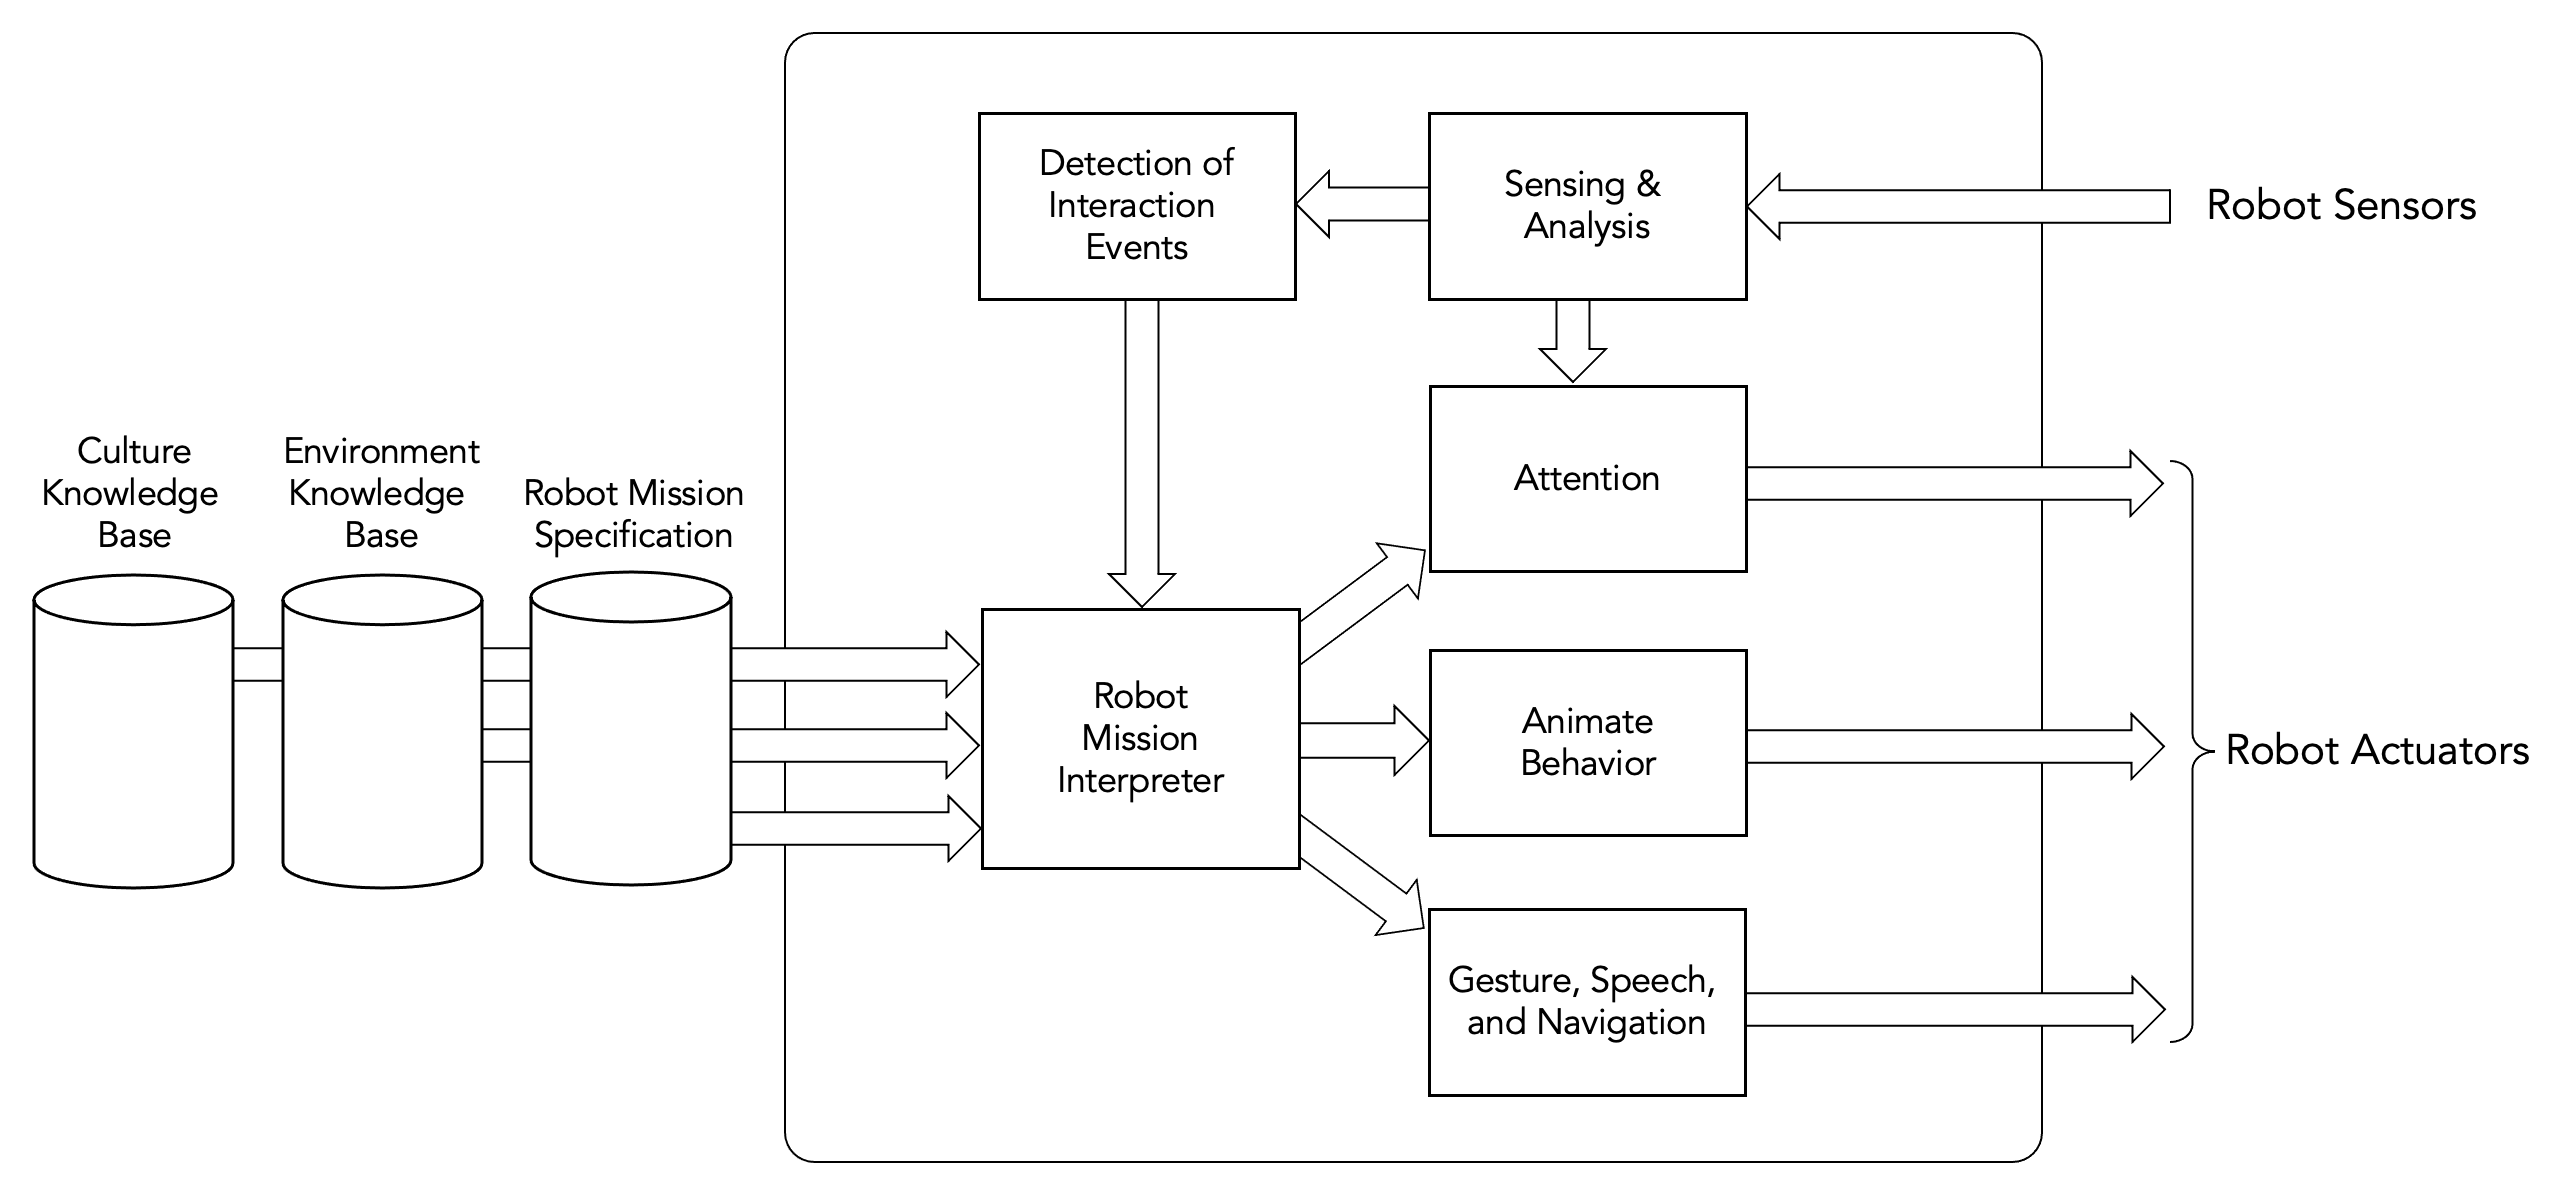
\includegraphics[width=160mm,angle=0]{System_Architecture.png}
\end{center}
\vspace{-5mm}
\caption{The CSSR4Africa system architecture.}  
\label{fig:architecture1}       
\end{figure}


\section{System Architecture Overview}
%###############################

The CSSR4Africa system architecture comprises six subsystems, as follows; also see Figure \ref{fig:architecture1}.
\begin{enumerate}
\item Sensing and Analysis
\vspace{-2mm}
\item Detection of Interaction Events
\vspace{-2mm}
\item Animate Behavior
\vspace{-2mm}
\item Attention
\vspace{-2mm}
\item Robot Mission Interpreter
\vspace{-2mm}
\item Gesture, Speech, \& Navigation
\end{enumerate}
Each subsystem comprises one or more ROS nodes, as shown in Table \ref{table:nodes}, with thirteen ROS nodes in total.
We provide a detailed specification of each ROS node in the following section.
All thirteen nodes are part of the  {\small \verb+cssr_system+}   ROS package; see Deliverable D3.2 Fig. 4 and Table 1.

\begin{table}[thb]
\begin{center}
\begin{tabular}{|l |l|}
\hline 
 {\small Subsystem  }                                         &  {\small ROS Node }      \\
\hline
{\small Sensing and Analysis }	              & {\footnotesize \verb+faceDetection+} \\
                                                             &  {\footnotesize \verb+personDetection+}  \\
                                                             & {\footnotesize \verb+soundDetection+}  \\
\hline
{\small Detection of Interaction Events} & {\footnotesize \verb+speechEvent+} \\
                                                             & {\footnotesize \verb+tabletEvent+} \\
\hline
{\small Robot Mission Interpreter }                 &  {\footnotesize \verb+behaviorController+}  \\
\hline
{\small Attention}                                  & {\footnotesize \verb+overtAttention+} \\
\hline
{\small Animate Behavior }	              & {\footnotesize \verb+animateBehavior+} \\

\hline
{\small Gesture, Speech, \& Navigation} & {\footnotesize \verb+gestureExecution+} \\
                                                              & {\footnotesize \verb+robotLocalization+}  \\
                                                              & {\footnotesize \verb+robotNavigation+}  \\
                                                              & {\footnotesize \verb+textToSpeech+} \\
\hline
\end{tabular}
\end{center}
\caption{The thirteen ROS nodes that comprise the six subsystems in the CSSR4Africa culturally-sensitive human-robot interaction software system.}
\label{table:nodes}
\end{table}
  

\newpage

\section{ROS Node Specifications}
%###############################
\label{section:nodes} 

\subsection{Animate Behavior}
%=================================================================================

\subsubsection*{ROS Node Name}
%----------------------------
 {\small \verb+animateBehavior+}   


\subsubsection*{Functional Specification}
%--------------------------------
This ROS node  gives the robot the appearance of an animate agent by continually making subtle  body  movements, flexing its hands a little, and rotating its base slightly.  

The node actuates the robot joints periodically in a random pattern, keeping the joint angles close to the default home positions. All the joints, except \verb+headYaw+ and \verb+headPitch+, are actuated, as well as the wheels to effect rotation about the robot's $z$-axis, but not forward movement along the robot's $x$-axis. The {\small \verb+headYaw+} and {\small \verb+headPitch+} joints are actuated by the {\small \verb+attention+} node.   The extent of the movements is determined by an external parameter. Specifically, the range of movement, from which the actual movement will be  a random sample, will be specified as a percentage of one tenth the full range of movement.  Thus, 10\%  means that the amount of motion will vary randomly between the home value and half the maximum value, assuming the home value is midway between the minimum and maximum values.  

The names of the topics to be used for each actuator are read from a data file comprising a sequence of key-value pairs. The key is the name of the actuator. The value is the topic name.  There are two data files, one for the physical robot and another for the simulator.  

To ensure that  the robot does not make these animate movements when engaged in culturally sensitive social interaction through gestures, speech, or when navigating, the generation of animate behavior is enabled and disabled by the Robot Mission Interpreter  subsystem using  a dedicated ROS service which the {\small \verb+animateBehavior+}   node advertizes and serves.

Any of the three types of animate behavior --- body movement, hand flex, and rotation --- can be selectively invoked. All three will be invoked if none are selectively invoked.

The node can run in normal mode or verbose mode. In verbose mode, data that is published to topics is also printed to the terminal.

\subsubsection*{Configuration File}
%-----------------------------

The operation of the {\small \verb+animateBehavior+} node is determined by the contents of a configuration file, {\small \verb+animateBehaviorConfiguration.ini+}, that  contains a list of key-value pairs as shown below.  

\begin{center}
\begin{tabularx}{\linewidth}{| l | l | X|}
\hline 
{\small Key }                               & {\small Values }                                                 &  {\small Effect}       \\
\hline
{\footnotesize \verb+platform+ }  & {\footnotesize \verb+robot+, \verb+simulator+}     & {\small Specifies the platform on which the node is to be run, i.e., the physical Pepper robot or the Pepper simulator} \\ 
\hline
{\footnotesize \verb+behavior+ }  & {\footnotesize \verb+body+, \verb+hands+, \verb+rotation+}     & {\small Specifies the type of animate behavior to exhibit.} \\ 
\hline
{\footnotesize \verb+range+ }  & {\footnotesize \verb+<number>+}     & {\small Specifies the range of actuator movement as a percentage of half the full range of movement.} \\
\hline
{\footnotesize \verb+robotTopics+ }  & {\footnotesize \verb+pepperTopics.dat+}     & {\small Specifies the filename of the file in which the physical Pepper robot sensor and actuator topic names are stored.} \\
\hline
{\footnotesize \verb+simulatorTopics+}  & {\footnotesize \verb+simulatorTopics.dat+}     & {\small Specifies the filename of the file in which the simulator  sensor and actuator topic names are stored.} \\
\hline
{\footnotesize \verb+verboseMode+}  & {\footnotesize \verb+true+, \verb+false+}     & {\small Specifies whether diagnostic data is to be printed to the terminal.} \\
\hline
\end{tabularx}
\end{center}

\subsubsection*{Input Data File}
%--------------------------
This node does not read from an input data file.


\subsubsection*{Output Data File}
%----------------------------
This node does not write to an output data file.


\subsubsection*{Topics Subscribed}
%-----------------------------
This node does not subscribe to any topics.


\subsubsection*{Topics Published}
%----------------------------
This node publishes on several actuator topics which are identified in the file given by the {\small \verb+robotTopics+ }  and {\small \verb+simulatorTopics+}  key-value pairs in the configuration file.
The following are the topics to which the {\small \verb+animateBehavior+} node publishes.
 
\begin{center}
\begin{tabularx}{\linewidth}{| X | l| l|}
\hline 
{\small Topic }                                                                                & {\small Actuator }    &  {\small Platform}       \\
\hline
{\footnotesize \verb+/pepper_dcm/RightHand_controller/+ }  & {\footnotesize  \verb+RHand+} & {\small Physical robot } \\ 
{\footnotesize \verb+follow_joint_trajectory+ }                        &   & \\ 
\hline
{\footnotesize \verb+/pepper_dcm/LeftHand_controller/+ }  & {\footnotesize \verb+LHand+ } & {\small Physical robot } \\ 
{\footnotesize \verb+follow_joint_trajectory+ }  & & \\ 
\hline
{\footnotesize \verb+/pepper_dcm/RightArm_controller/+ }  & {\footnotesize \verb+RShoulderPitch+, \verb+RShoulderRoll+,   } & {\small Physical robot } \\ 
{\footnotesize \verb+follow_joint_trajectory+ }                                          & {\footnotesize \verb+RElbowYaw+, \verb+RElbowRoll+, \verb+RWristYaw+  } & \\
\hline
{\footnotesize \verb+/pepper_dcm/LeftArm_controller/+ }     & {\footnotesize  \verb+LShoulderPitch+, \verb+LShoulderRoll+,  } & {\small Physical robot } \\ 
{\footnotesize \verb+follow_joint_trajectory+ }                                        & {\footnotesize  \verb+LElbowYaw+, \verb+LElbowRoll+, \verb+LWristYaw+  } & \\ 
\hline
{\footnotesize \verb+/pepper_dcm/Pelvis_controller/+ }  & {\footnotesize \verb+HipRoll+, \verb+HipPitch+,  \verb+KneePitch+ } & {\small Physical robot } \\ 
{\footnotesize \verb+follow_joint_trajectory+ }                                   & {\footnotesize  } & \\ 
\hline
{\footnotesize \verb+/cmd_vel+ }  & {\footnotesize \verb+WheelFL+, \verb+WheelFR+, \verb+WheelB+ } & {\small Physical robot } \\ 
\hline
{\footnotesize \verb+/pepper/RightArm_controller/+ }  & {\footnotesize \verb+RElbowYaw+, \verb+RElbowRoll+ } & {\small  Simulator} \\ 
{\footnotesize \verb+follow_joint_trajectory+ }                        &   & \\ 
\hline
{\footnotesize \verb+/pepper/LeftArm_controller/+ }  & {\footnotesize  \verb+LElbowYaw+, \verb+LElbowRoll+ } & {\small  Simulator} \\ 
{\footnotesize \verb+follow_joint_trajectory+ }                        &   & \\ 
\hline
{\footnotesize \verb+/pepper/Pelvis_controller/+ }  & {\footnotesize \verb+HipRoll+, \verb+HipPitch+, \verb+KneePitch+ } & {\small  Simulator} \\ 
{\footnotesize \verb+follow_joint_trajectory+ }                        &   & \\ 
\hline
{\footnotesize \verb+/pepper/cmd_vel+ }  & {\footnotesize \verb+WheelFL+, \verb+WheelFR+, \verb+WheelB+ } & {\small  Simulator} \\ 
\hline
\end{tabularx}
\end{center}
 

\subsubsection*{Services Supported}
%---------------------------------------
This node  provides and advertizes a server for a service {\small \verb+/animateBehavior/set_activation+} to enable and disable the operation of the node, i.e., to activate or suspend the publishing of data on the actuator topics to give the appearance of an animate agent.  It uses a package-specific msg, {\small \verb+State.msg+} with just one field  {\small \verb+string state+}, with a value of either ``{\small \verb+enabled+}'' or ``{\small \verb+disabled+}''. Depending on the string value, {\small \verb+animateBehavior+} will be enabled or disabled.  If the enable/disable request is successful, the service response is ``1''; if it is unsuccessful, it is ``0''.  
The service is called by  the {\small \verb+behaviorController+} node, enabling or disabling animate behavior, as needed.

The following summarizes the services supported.

\begin{center}
\begin{tabularx}{\linewidth}{| l | l | X|}
\hline 
{\small Service }                                                                                & {\small Message Value}    &  {\small Effect}       \\
\hline
{\footnotesize \verb+/animateBehavior/set_activation+ }  & {\footnotesize \verb+enabled+,   \verb+disabled+ } & {\small Enable or disable animate behavior} \\ 
\hline
\end{tabularx}
\end{center}


\subsubsection*{Services Called}
%---------------------------------------
This node does not call any services.



\newpage

\subsection{Behavior Controller}
%=================================================================================
\label{section:behavior_controller}

\subsubsection*{ROS Node Name}
%----------------------------
 {\small \verb+behaviorController+}   

\subsubsection*{Functional Specification}
%--------------------------------
This ROS node  provides that interprets the robot mission language developed in Task 5.4.2 and implements the specification of the two  use case scenarios in that language, as documented in Deliverable D5.4.2. In does so by  recruiting the robot and visitor behaviors documented in Deliverables D2.2 and D2.3, and the cultural knowledge encapsulated in Deliverable D5.4.1, and realized in the robot sensing modules developed in Work Package 4 and the robot behavior modules developed in Work Package 5.  The outcome of this task  is described in Deliverable D5.4.3. 

The dynamics of interaction between the robot and the visitor in the two use case scenarios are specified by robot mission specifications  written in the robot mission language defined in Task 5.4.2.  The  {\small \verb+behaviorController+}  node interacts with other CSSR4Africa ROS nodes to realize these dynamics.  It does this by calling various services. These are detailed below.

The node can run in normal mode or verbose mode. In verbose mode, data that is published to topics is also printed to the terminal.

\subsubsection*{Configuration File}
%-----------------------------

The operation of the {\small \verb+behaviorController+} node is determined by the contents of a configuration file,  {\small \verb+behaviorControllerConfiguration.ini+},  that  contain a list of key-value pairs as shown below.  
 
\begin{center}
\begin{tabularx}{\linewidth}{| l | l | X|}
\hline 
{\small Key }                               & {\small Values }                                                 &  {\small Effect}       \\
\hline
{\footnotesize \verb+scenarioSpecification+}  & {\footnotesize \verb+scenarioSpecification.dat+}     & {\small Specifies the filename of the file in which the robot mission specificatgion is stored.} \\
\hline
{\footnotesize \verb+verboseMode+}  & {\footnotesize \verb+true+, \verb+false+}     & {\small Specifies whether diagnostic data is to be printed to the terminal.} \\
\hline
\end{tabularx}
\end{center}

\subsubsection*{Input Data File}
%--------------------------
This node reads the interaction scenario robot mission specification file specified in the configuration file.


\subsubsection*{Output Data File}
%----------------------------
This node does not write to an output data file.


\subsubsection*{Topics Subscribed}
%-----------------------------
This node  subscribes to three topics, as follows. 

\begin{center}
\begin{tabularx}{\linewidth}{| l | l | X|}
\hline 
{\small Topic }                               & {\small Node }                            &  {\small Platform}       \\
\hline
{\footnotesize \verb+/speechEvent/text+ }  & {\footnotesize \verb+speechEvent+}    & {\small Physical robot  } \\ 
\hline
{\footnotesize \verb+/robotLocalization/pose+ }  & {\footnotesize \verb+/robotLocalization+}    & {\small Physical robot  } \\ 
\hline
{\footnotesize \verb+/personDetection/data+ }  & {\footnotesize \verb+/personDetection+}    & {\small Physical robot  } \\ 
\hline
\end{tabularx}
\end{center}
The {\small \verb+/robotLocalization/pose+}  and {\small \verb+/personDetection/data+} topics are needed to allow navigation with respect to people in the robot's field of view.

\subsubsection*{Topics Published}
%----------------------------
This node does not publish to any  topics.


\subsubsection*{Services Supported}
%---------------------------------------

This node does not provide and advertize  any services.

\subsubsection*{Services Called}
%---------------------------------------
\label{section:robot_mission_interpreter_services_called}

This node  calls the following services to implement the interaction dynamics specified in the scenario robot mission specification.

\begin{center}
\begin{tabularx}{\linewidth}{| l | l | X|}
\hline 
{\small Service }                                                    & {\small Message Value}    &  {\small Effect}       \\
\hline
 {\footnotesize \verb+/animateBehavior/set_activation+} & {\small To be defined} &  {\small Enable and disable the operation of} {\footnotesize \verb+animateBehavior+} \\
\hline
 {\footnotesize \verb+/gestureExecution/perform_gesture+} & {\small To be defined} &  {\small Initiate the performance of a required gesture}\\
\hline
%%{\footnotesize \verb+/knowledgeBase/query+ }  & {\small To be defined} & {\small Extract required knowledge from the cultural knowledge base} \\ 
%%\hline
{\footnotesize \verb+/overtAttention/set_mode+} & {\small To be defined} &  {\small Set the social, scanning, or location mode of attention}\\
%%\hline
%%{\footnotesize \verb+/overtAttention/set_activation+} & {\small To be defined} &  {\small Enable and disable the operation of} {\footnotesize \verb+overtAttention+}\\
\hline
{\footnotesize \verb+/robotNavigation/set_goal+}  &  {\footnotesize \verb+<x>+ \verb+<y>+  \verb+<theta>+}  & {\small Navigate to a given location} \\ 
\hline
{\footnotesize \verb+/robotLocalization/set_pose+ }  & {\footnotesize \verb+<x>+ \verb+<y>+  \verb+<theta>+}  & {\small Set robot pose} \\ 
\hline
{\footnotesize \verb+/tabletEvent/prompt_and_get_response+} &{\small To be defined} &  {\small Seek input from the visitor}\\
\hline
{\footnotesize \verb+/textToSpeech/say_text+ }  & {\footnotesize \verb+<string>+} & {\small Say a text message} \\ 

\hline
\end{tabularx}
\end{center}

The type of the variables that are passed as an argument to the service calls  has not yet been defined. This will be done when the node that services and advertizes these services are fully specified.
Similarly, the type of the service call  return value has not yet been defined. Again, this will be done when the node that services and advertizes these services are fully specified.


\subsubsection*{Helper Classes Used}
%---------------------------------------
This node  uses an instantiation of a helper class {\small \verb+CultureKnowledgeBase+}  to read the culture knowledge base file and retrieve the required data using  class access methods. 

Similarly, it uses  an instantiation of a helper class {\small \verb+EnvironmentKnowledgeBase+}  to read the environment knowledge base file and retrieve the required data using  class access methods.  


The type of the variables that are passed as  arguments to the 
%%\small \verb+/knowledgeBase/query+}  service   
{\small \verb+CultureKnowledgeBase+} helper class access methods and the 
{\small \verb+EnvironmentKnowledgeBase+} helper class access methods 
have not yet been defined. 
These will be done when the helper classes are fully specified in Deliverables D5.4.1 and D5.4.2, respectively.
%%node that services and advertizes these services are fully specified.
%%Similarly, the type of the service call  return value has not yet been defined. Again, this will be done when the node that services and advertizes these services are fully specified.


\newpage

\subsection{Face Detection }
%=================================================================================

\subsubsection*{ROS Node Name}
%----------------------------
 {\small \verb+faceDetection+}   

\subsubsection*{Functional Specification}
%--------------------------------
This ROS node detects faces and their location  in the field of view of the Pepper robot and  and determine their gaze direction. It computes their position in an 2D image frame of reference. In addition, the region that the face occupies in the image is determined by computing the bounding box surrounding the face. If more than one face is present in the robot’s field of view, then all of them are detected and localized.  

To ensure coherence in detection and localization over time, each detected face is labelled (e.g., ``Face 1'') and the same label is assigned to that person in subsequent images.  The label and the bounding box are be colour-coded, assigning different colours to different faces, and the same colour to a given face in each image in a sequence of images.   If that face is no longer detected in one or more images  (the number to be specified in a configuration parameter value) due to, for example, a false reject error, then that label is not reused. If that face reappears in a subsequent image, it is given a new label. As such, this module is only concerned with consistent detection of face over time, not recognition of previously detected face, and it is assumed that people don't change between images.  Consequently, a face detected in one image is deemed to be the same as one in a previous image if the spatial displacement between their centroids is within a defined tolerance or the Intersection over Union (IoU) between their bounding boxes exceeds a specified threshold defined in the configuration parameters.

Additionally, for each detected face, the ROS node assesses whether the person is gazing directly at the robot. This is accomplished using head pose estimation, which provides a simpler alternative to mutual gaze detection.

The node has two inputs: an RGB image and a depth image from either the robot’s cameras or the Intel realsense camera. In addition, there is an option to use compressed images instead of raw image for both RGB and depth image.

The node has three outputs: an RGB image, with bounding boxes drawn around each detected face in the RGB images, depth image and an array of  records (one record for each face detected).  

Each record consists of the face label, the 3D image coordinates representing the centroid of the bounding box, the distance (or depth) of the face from the camera based on the centroid, a Boolean value indicating whether mutual gaze is established between the corresponding face and the Pepper robot, and the width and height of the face bounding box.

The image is displayed in an openCV window when the node is operating in verbose mode.  The array of records is  published to a  topic named {\small \verb+/faceDetection/data+}.
 
The names of the topics to be used for each camera is read from a data file comprising a sequence of key-value pairs. The key is the name of the camera. The value is the topic name.    

The node can run in normal mode or verbose mode. In verbose mode, data that is published to topics is also printed to the terminal, and output images are also displayed in openCV windows.

\newpage

\subsubsection*{Configuration File}
%-----------------------------


The operation of the {\small \verb+faceDetection+} node is determined by the contents of a configuration file, {\small \texttt{faceDetectionConfiguration.json}, that  contain a list of key-value pairs as shown below.  

\begin{center}
\begin{tabularx}{\linewidth}{| l | l | X|}
\hline
{\footnotesize \texttt{algorithm} }  & {\footnotesize \texttt{mediapipe}, \texttt{sixdrep}}   & {\small Specifies which algorithm to use.} \\
\hline
%=============
%{\footnotesize \texttt{\textcolor{red}{angleThreshold}} }  & {\footnotesize \texttt{<number>}}  & {\small Specifies the maximum angular deviation (in degrees) for mutual gaze detection.} \\
%\hline
%{\footnotesize \texttt{\textcolor{red}{falseRejectTolerance}} } & {\footnotesize \texttt{<number>}} & {\small Specifies the number of images in which a face is not detected before it will be assigned a new label if and when it reappears at the same location. For example, a value of 1 indicates that if the face is not detected in one image but reappears at that location in the next, it will be assigned the same label.} \\
%\hline
%{\footnotesize \texttt{\textcolor{red}{spatialTolerance}} } & {\footnotesize \texttt{<number>}} & {\small Specifies the spatial tolerance, given as a percentage of the width of the image.} \\
%\hline
%=============
{\footnotesize \texttt{useCompressed} }  & {\footnotesize \texttt{<true or false>}}     & {\small Specifies to use compressed images or raw images.} \\
\hline
{\footnotesize \texttt{mpFacedetConfidence} }  & {\footnotesize \texttt{<number>}}     & {\small Specifies the confidence threshold for the MediaPipe face detection algorithm.} \\
\hline
{\footnotesize \texttt{mpHeadposeAngle} }  & {\footnotesize \texttt{<number>}}     & {\small Specifies the maximum angular deviation (in degrees) for MediaPipe head pose estimation.} \\
\hline
{\footnotesize \texttt{centroidMaxDistance} }  & {\footnotesize \texttt{<number>}}     & {\small Specifies the maximum allowed distance (in pixels) between centroids for tracking continuity.} \\
\hline
{\footnotesize \texttt{centroidMaxDisappeared} }  & {\footnotesize \texttt{<number>}}     & {\small Specifies the maximum number of frames a centroid can disappear before being considered lost.} \\
\hline
{\footnotesize \texttt{sixdrepnetConfidence} }  & {\footnotesize \texttt{<number>}}     & {\small Specifies the confidence threshold for the SixDRepNet pose estimation algorithm.} \\
\hline
{\footnotesize \texttt{sixdrepnetHeadposeAngle} }  & {\footnotesize \texttt{<number>}}     & {\small Specifies the maximum angular deviation (in degrees) for SixDRepNet head pose estimation.} \\
\hline
{\footnotesize \texttt{sortMaxDisappeared}}  & {\footnotesize \texttt{<number>}}     & {\small Specifies the maximum number of frames an object can disappear for SORT tracker before being removed.} \\
\hline
{\footnotesize \texttt{sortMinHits}}  & {\footnotesize \texttt{<number>}}     & {\small Specifies the minimum number of consecutive hits required for SORT tracker initialization.} \\
\hline
{\footnotesize \texttt{sortIouThreshold}}  & {\footnotesize \texttt{<number>}}     & {\small Specifies the Intersection over Union (IoU) threshold for SORT tracker associations.} \\
\hline
{\footnotesize \texttt{verboseMode}}  & {\footnotesize \texttt{<true or false>}}     & {\small Specifies whether diagnostic data is to be printed to the terminal and diagnostic images are to be displayed in OpenCV windows.} \\
\hline
\end{tabularx}
\end{center}


\subsubsection*{Input Data File}
%--------------------------
This node does not read from an input data file.


\subsubsection*{Output Data File}
%----------------------------
This node does not write to an output data file.

\subsubsection*{Topics Subscribed}
%-----------------------------

This node subscribes to four topics: two RGB camera sensor topics (one published by the Pepper robot, one by the RealSense camera), and two depth camera topics (one published by the Pepper robot, one by the RealSense camera).
These are specified in the files identified by the {\small \verb+robotTopics+ }  key-value pair in the configuration file.

\newpage

The following are the topics to which the \texttt{\small faceDetection}  node subscribes.

\begin{table}[!h]
	\centering
	{\fontsize{8.2}{11.0}\selectfont % <- apply inside the table
		\begin{tabularx}{\linewidth}{| l | l | X |}
			\hline
			\small{Topic} & \small{Sensor / Node} & \small{Platform} \\
			\hline
			\texttt{/camera/color/image\_raw} & \texttt{RGBRealSense} & Intel RealSense \\
			\hline
			\texttt{/camera/color/image\_raw/compressed} & \makecell[l]{\texttt{RGBRealSense} \\ (Compressed)} & Intel RealSense \\
			\hline
			\texttt{/camera/aligned\_depth\_to\_color/image\_raw} & \texttt{DepthRealSense} & Intel RealSense \\
			\hline
			\texttt{/camera/aligned\_depth\_to\_color/image\_raw/compressed} & \makecell[l]{\texttt{DepthRealSense} \\ (Compressed)} & Intel RealSense \\
			\hline
			\texttt{/naoqi\_driver/camera/front/image\_raw} & \texttt{FrontCamera} & Physical Robot (Pepper) \\
			\hline
			\texttt{/naoqi\_driver/camera/depth/image\_raw} & \texttt{DepthCamera} & Physical Robot (Pepper) \\
			\hline
		\end{tabularx}
	}
\end{table}



\subsubsection*{Topics Published}
%----------------------------

The following are the topics which the \small \texttt{faceDetection}   node publishes.
 
\begin{center}
\begin{tabularx}{\linewidth}{| l | l | X|}
\hline 
{\small Topic }                                                                                & {\small Sensor / Actuator / Node}    &  {\small Platform}       \\
\hline
{\footnotesize \verb+/faceDetection/data+ }  & {\footnotesize \verb+overtAttention+, \verb+GUI+ } & {\small Physical robot} \\ 
\hline
\end{tabularx}
\end{center}

\subsubsection*{Services Supported}
%---------------------------------------
This node  does not support any services.

\subsubsection*{Services Called}
%---------------------------------------
This node does not call any services.






 
\newpage

\subsection{Gesture Execution }
%=================================================================================

\subsubsection*{ROS Node Name}
%----------------------------
 {\small \verb+gestureExecution+}   

\subsubsection*{Functional Specification}
%--------------------------------
This ROS node  provides the robot with the ability to execute five forms of gesture: deictic, symbolic, and iconic non-verbal hand gestures, and bowing and nodding body gestures. 
 
The specifications for these gestures are in joint space, except for deictic gestures which are  in Cartesian space.  Some gestures, e.g., iconic and symbolic hand gestures, are specified by learning the required motions either by manual teleoperation, recording the joint angles, or by demonstration,  using an RGB-D depth camera to determine the joint angles of human gestures in a skeletal model  and mapping  these to the robot joints. Other gestures, i.e., deictic hand gestures and body gestures, are specified by gesture parameters, such as the pointing location for deictic gestures and the degree of inclination for bowing and nodding, and the joint angles are computed using the kinematic model of the robot head, torso, and arms. For deictic gestures, which require the robot to point at objects in its environment and move its head to look at the object, the pose of the robot in the world frame of reference is also used.
 
If the arm cannot achieve the required pose for a deictic gesture, the robot  rotates to make the pose achievable, returning to the original orientation once the gesture is complete.  Futhermore, the arm  returns to a neutral position by the robot's side when the gesture is complete.

Iconic and symbolic gestures are defined by descriptors that specify the final gesture joint configuration and the manner in which that configuration is achieved.  
Descriptors comprise four elements. Each element is a key-value pair, where the value can be an identifier, a number, a vector of numbers, or a vector of a vector of numbers. 

The first key-value pair  specifies  the gesture type (e.g., {\small \verb+type iconic+}, {\small \verb+type symbolic+}).  

The second key-value pair  identifies the  ID number (e.g., {\small \verb+ID 01+}).

The third element defines the number of waypoints in the trajectory, including the start gesture joint configuration and  the final gesture joint configuration.  

The fourth element is a vector of joint angles vectors. The number of joint angle vectors is equal to the number of way points, including the start joint configuration and the final gesture configuration.  Body gestures have three joints: knee pitch, hip pitch, hip roll. Iconic and symbolic gestures have five joints: shoulder pitch, shoulder roll, elbow yaw, elbow roll, and wrist yaw. Before beginning the gesture, the arm is moved from its current joint configuration to the start joint configuration, i.e., the joint angles specified in the first vector in the vector of vector of joint angles.  

The number of elements in the vector of joint angles is determined by the gesture type. 

Descriptors for each gesture are stored in an external descriptor file. 
 
If an iconic or symbolic gesture involves two arms, they are treated as a composite of two individual gestures, one for each arm.
 
The joint angles for bow and nod body gestures, as well as hand deictic gestures,  are computed at run time using the kinematic model of the robot and the bow angle, nod angle, or the location in the environment to which the robot should point.  
The bow angle, nod angle, and pointing location  are provided as an input to the module, along with the time  in milliseconds that should elapse between the start of the gesture and the end of the gesture. 

The pointing location  with respect to the robot body, specified by the shoulder pitch and shoulder roll angles, is computed from the pointing location in the world frame of reference (and supplied as an input to the module) and the pose of the robot in the world frame of reference (provided by the {\small \verb+robotLocalization+} node.   
No waypoints are required for deictic gestures; the joints are actuated to achieve the target joint angles, interpolating linearly, or adjusting the joint angles, joint angular velocities, and joint accelerations to mimic biological movement by using a minimum jerk model of biological motion. 

It is assumed that the knee pitch angle is fixed during a bow body gesture and that the bow angle corresponds to the change in the hip pitch angle with respect to the default hip pitch angle.   Similarly, it is assumed that the nod angle is the change in the head pitch angle with respect to the default head pitch angle.  Finally, it is assumed that the arm and fingers are  straight in a deictic gesture, with fixed values of elbow yaw, elbow roll,  wrist yaw, and hand angles, so that the palm of the hand is directed upwards.
 
The input to the module is a record comprising  the gesture type (e.g., {\small \verb+iconic+}, {\small \verb+symbolic+}, {\small \verb+deictic+}, {\small \verb+bow+}, {\small \verb+nod+}), the gesture ID for symbolic or iconic gestures (e.g., {\small \verb+01+}), the duration of the gesture in milliseconds, and either  a bow angle in degrees (for a bow body gesture), or a nod angle in degrees (for  a nod body gesture), or  the  three dimensional coordinates of a pointing location (for a deictic gesture).  For deictic gestures, the module also inputs the current robot pose from the {\small \verb+robotLocalization+} node. 

The output is a sequence of joint angles, joint angular velocities, and, optionally, joint angular accelerations. Data is published on the appropriate topics, as required.
 
The names of the topics to be used for each actuator is read from a data file comprising a sequence of key-value pairs. The key is the name of the actuator. The value is the topic name.    

The node can run in normal mode or verbose mode. In verbose mode, data that is published to topics is also printed to the terminal.


\subsubsection*{Configuration File}
%-----------------------------

The operation of the {{\small \verb+gestureExecution+} node is determined by the contents of a configuration file,\\ {\small \verb+gestureExecutionConfiguration.ini+}, that contains a list of key-value pairs, as shown below.

\begin{center}
\begin{tabularx}{\linewidth}{| l | l | X|}
\hline 
{\small Key }                               & {\small Values }                                                 &  {\small Effect}       \\
\hline
{\footnotesize \verb+interpolation+ }  & {\footnotesize \verb+linear+, \verb+biological+}     & {\small Specifies the interpolation type. This indicates how the joint angles that define the trajectory in joint space between the current joint angles and the gesture joint angles are computed for body gesture and hand deictic gestures, and between way points for iconic and symbolic gestures. The two options are: (a) independent linear  interpolation of each joint angle, and (b)  biological motion, selecting  the sequence of  joint angular velocities and joint accelerations  to form a trajectory in time and joint space that mimics biological movement.}\\ 
\hline
{\footnotesize \verb+gestureDescriptors+ }  & {\footnotesize \verb+gestureDescriptors.dat+}     & {\small Specifies the  filename of the file in which the gesture descriptors are stored.} \\ 
\hline
{\footnotesize \verb+robotTopics+ }  & {\footnotesize \verb+pepperTopics.dat+}     & {\small Specifies the filename of the file in which the physical Pepper robot sensor and actuator topic names are stored.} \\
\hline
{\footnotesize \verb+verboseMode+}  & {\footnotesize \verb+true+, \verb+false+}     & {\small Specifies whether diagnostic data is to be printed to the terminal.} \\
\hline
\end{tabularx}
\end{center}


\subsubsection*{Input Data File}
%--------------------------
This node does not read from an input data file.


\subsubsection*{Output Data File}
%----------------------------
This node does not write to an output data file.

\newpage

\subsubsection*{Topics Subscribed}
%-----------------------------
This node  subscribes to one topic, published by {\small \verb+robotLocalization+} node, which provides the pose of the robot.

The following are the topics to which the {\small \verb+gestureExecution+} node subscribes.

\begin{center}
\begin{tabularx}{\linewidth}{| l | l | X|}
\hline 
{\small Topic }                               & {\small Node }                            &  {\small Platform}       \\
\hline
{\footnotesize \verb+/robotLocalization/pose+ }  & {\footnotesize \verb+robotLocalization+}    & {\small Physical robot} \\ 
\hline
\end{tabularx}
\end{center}


\subsubsection*{Topics Published}
%----------------------------

The following are the topics to which the {\small \verb+gestureExecution+} node publishes.
These are specified in the file identified by the {\small \verb+robotTopics+ }    key-value pair in the configuration file.

\begin{center}
\begin{tabularx}{\linewidth}{| X | l| l|}
\hline 
{\small Topic }                                                                                & {\small Actuator }    &  {\small Platform}       \\
\hline
{\footnotesize \verb+/pepper_dcm/RightHand_controller/+ }  & {\footnotesize  \verb+RHand+} & {\small Physical robot } \\ 
{\footnotesize \verb+follow_joint_trajectory+ }                        &   & \\ 
\hline
{\footnotesize \verb+/pepper_dcm/LeftHand_controller/+ }  & {\footnotesize \verb+LHand+ } & {\small Physical robot } \\ 
{\footnotesize \verb+follow_joint_trajectory+ }  & & \\ 
\hline
{\footnotesize \verb+/pepper_dcm/RightArm_controller/+ }  & {\footnotesize \verb+RShoulderPitch+, \verb+RShoulderRoll+,   } & {\small Physical robot } \\ 
{\footnotesize \verb+follow_joint_trajectory+ }                                          & {\footnotesize \verb+RElbowYaw+, \verb+RElbowRoll+, \verb+RWristYaw+  } & \\
\hline
{\footnotesize \verb+/pepper_dcm/LeftArm_controller/+ }     & {\footnotesize  \verb+LShoulderPitch+, \verb+LShoulderRoll+,  } & {\small Physical robot } \\ 
{\footnotesize \verb+ follow_joint_trajectory+ }                                        & {\footnotesize  \verb+LElbowYaw+, \verb+LElbowRoll+, \verb+LWristYaw+  } & \\ 
\hline
{\footnotesize \verb+/pepper_dcm/Pelvis_controller/+ }  & {\footnotesize \verb+HipRoll+, \verb+HipPitch+,  \verb+KneePitch+ } & {\small Physical robot } \\ 
{\footnotesize \verb+follow_joint_trajectory+ }                                   & {\footnotesize  } & \\ 
\hline
{\footnotesize \verb+/cmd_vel+ }  & {\footnotesize \verb+WheelFL+, \verb+WheelFR+, \verb+WheelB+ } & {\small Physical robot } \\ 
\hline
\end{tabularx}
\end{center}
 

\subsubsection*{Services Supported}
%---------------------------------------
 This node  provides and advertizes a server for a service {\small \verb+/gestureExecution/perform_gesture+} to initiate the performance of a required gesture. It uses a package-specific msg, {\small \verb+Gesture.msg+}.
The message has several fields, as follows.

\begin{center}
\begin{tabularx}{\linewidth}{| l | X | l| l|}
\hline 
{\small Field }                                                                                & {\small Field Value}    &  {\small Field Type}  &     {\small Units}   \\
\hline
{\footnotesize  \verb+gesture_type+}  & {\footnotesize \verb+iconic+,   \verb+symbolic+, \verb+deictic+, \verb+bow+, \verb+nod+   } & {\small String} & \\ 
\hline
{\footnotesize  \verb+gesture_id+}  & {\footnotesize \verb+<number>+    } & {\small Integer}  & \\ 
\hline
{\footnotesize  \verb+gesture_duration+}  & {\footnotesize \verb+<number>+    } & {\small Integer} & {\footnotesize milliseconds} \\ 
\hline
{\footnotesize  \verb+bow_nod_angle+}  & {\footnotesize \verb+<number>+    } & {\small Integer} & {\small degrees} \\ 
%\hline
%{\footnotesize  \verb+nod_angle+}  & {\footnotesize \verb+<number>+    } & {\small Integer} & {\small degrees} \\ 
\hline
{\footnotesize  \verb+location_x+}  & {\footnotesize \verb+<number>+    } & {\small Real} & {\small metres} \\ 
\hline
{\footnotesize  \verb+location_y+}  & {\footnotesize \verb+<number>+    } & {\small Real} & {\small metres} \\ 
\hline
{\footnotesize  \verb+location_z+}  & {\footnotesize \verb+<number>+    } & {\small Real} & {\small metres} \\ 
\hline
\end{tabularx}
\end{center}

If the {\small \verb+perform_gesture+} request is successful, the service response is ``1''; if it is unsuccessful, it is ``0''.  
The service  is called by  the {\small \verb+behaviorController+} node.
 
The following summarizes the services supported.

\begin{center}
\begin{tabularx}{\linewidth}{| l | l | X|}
\hline 
{\small Service }                                                                                & {\small Message Value}    &  {\small Effect}       \\
\hline
{\footnotesize \verb+/gestureExecution/perform_gesture+ }  & {\footnotesize \verb+iconic+,   \verb+symbolic+,   } & {\small Perform an iconic, symbolic, } \\ 
  & {\footnotesize  \verb+deictic+, \verb+bow+, \verb+nod+ } &    or deictic gesture \\ 
\hline
\end{tabularx}
\end{center}



\subsubsection*{Services Called}
%---------------------------------------
This node  invokes the service {\small \verb+/overtAttention/set_mode+} to move the robot's head to focus on the location required to gesture at. 

\begin{center}
	\begin{tabularx}{\linewidth}{| l | l | X|}
		\hline 
		{\small Service }                                                                                & {\small Message Value}    &  {\small Effect}       \\
		\hline
		{\footnotesize \verb+/overtAttention/set_mode+ }  & {\footnotesize \verb+location+} & {\small Move the head to focus on a location } \\ 
		& {\footnotesize  \verb+x+, \verb+y+, \verb+z+ } &    defined by the parameters \\ 
		\hline
	\end{tabularx}
\end{center}










\newpage

\subsection{Overt Attention }
%=================================================================================

\subsubsection*{ROS Node Name}
%----------------------------
 {\normalsize \verb+overtAttention+}   

\subsubsection*{Functional Specification}
%--------------------------------
This ROS node   provides the robot with the ability to direct the gaze of the robot  to salient features in the environment or to a given location in the environment. 

There are five modes of operation: a social mode, a scanning mode, a location mode, a seeking mode, and a disabled mode. The first is active when the robot is engaged in social interaction.  In this mode, the salient features are people's bodies, faces, eyes, and voices.  The second is active when the robot is not engaged in social interaction and it  is scanning the environment looking for people with whom to interact.  In this mode, the salient features also include objects of interest in the robot's environment, in addition faces. People's faces has a higher priority than other general features.  In the second mode of operation, the robot  switches its focus of attention after a short period of time and  does not return directly to the original focus of attention, thereby scanning its environment. In the third mode of operation, the robot gazes at a given location in its environment. If the head cannot achieve the required pose to gaze at a given location, the robot  rotates to make the pose achievable. In the fourth mode, seeking, the robot attempts to establish mutual gaze with a person nearby for a short duration, after which, if unsuccessful, it returns success or failure. To establish mutual gaze, the node searches for a face that is looking straight at the robot.  The robot might have to rotate about its base as well as rotating its head when searching. In disabled mode, the head is centred and remains immobile. The mode of operation is selected on the basis of a service request (see below).

Two saliency maps are  generated, one based on social features and one based on the combination of social and general conspicuous features. The first is based on  the output of  Task 4.2.2 Face \& Mutual Gaze Detection and Localization, and Task 4.2.3 Sound Detection and Localization. The second  is based on   information-theoretic saliency  and the output of Task 4.2.2 Face \& Mutual Gaze Detection and Localization \cite{BruceTsotsos09}. 

In the  scanning attention mode, three processes are active.
The first is a winner-take-all process to determine a single focus of attention from the candidates in the saliency map. This is effected by a selective tuning model \cite{Tsotsosetal95,Tsotsos06,Tsotsos11}.
The second is an Inhibition-of-Return (IOR) mechanism that attenuates the attention value of previous winning locations so that new regions become the focus of attention.
The third is an habituation process to gradually reduce the salience of the current focus of attention, thereby ensuring that attention is fixated on a given point only for a limited period \cite{ZaharescuRothensteinTsotsos05}. 

The robot's gaze is directed by publishing the appropriate  messages on the topic that controls the {\small \verb+headYaw+} and {\small \verb+headPitch+} joints so that the gaze is centred on the focus of attention.  This requires the calibration of the $x$ and $y$ offset of the focus of attention in the image to the change in {\small \verb+headYaw+} and {\small \verb+headPitch+} angles, respectively.  In the case of aural attention to conspicuous sounds, it requires the calibration of the angle of arrival  of the sound with the change in {\small \verb+headYaw angle+}.  Fixation on sounds will only control the {\small \verb+headYaw+} angle, i.e., rotation in the horizontal plane about the head's $z$-axis.  

These calibration constants are  provided as parameters to the node.  If the angle of rotation of the {\small \verb+headYaw+}  joint is greater than some threshold (defined as a parameter), then after rotating the head to fixate on the focus of attention, the base of the robot and the head  rotate in opposite directions so that the robot continues to gaze at the focus of attention while it realigns its head with its body.  The threshold for this head-torso realignment is provided as a parameter to the node.

The node has four inputs, all acquired by subscribing to the appropriate topics. These are the outputs of the  {\small \verb+faceDetection+} node and the {\small \verb+soundDetection+} node to be used to compute the saliency map in social mode, an RGB image from the robot's top forehead camera or the additional RealSense external camera to be used to compute the saliency map in scanning mode, and, when attending to a given location in the environment,  the current robot pose from the {\small \verb+robotLocalization+} node.
 
The node has four outputs, effected by publishing to the topic to control the {\small \verb+headYaw+} and {\small \verb+headPitch+} joints, and, if required, the topic to control robot's wheels and the robot's angular velocity when adjusting its pose to recentre the  gaze or enable the gaze to be directed at a given location. The third output is an RGB image depicting the saliency function and the selected focus of attention.  
The image is displayed in an openCV window when the node is operating in verbose mode (see below). The fourth output is the current active mode indicating which mode of operation the node is in at that moment. The mode is continuously published to the {\small \verb+/overtAttention/mode+} topic.

The names of the topics to be used for each actuator are read from a data file comprising a sequence of key-value pairs. The key is the name of the actuator. The value is the topic name.   

To ensure that  the robot does not  rotate to realign its head and torso when navigating, attention is disabled by the {\small \verb+behaviorController+} node using a dedicated service which the {\small \verb+overtAttention+} node advertizes and serves. It can also enable attention by setting the mode to social, seeking, scanning, or location mode also effected by the {\small \verb+overtAttention+} node using the same dedicated service which the {\small \verb+overtAttention+} node advertizes and serves.

The node can run in normal mode or verbose mode. In verbose mode, data that is published to topics is also printed to the terminal, and output images are also displayed in openCV windows.



\subsubsection*{Configuration File}
%-----------------------------

The operation of the {\small \verb+overtAttention+} node is determined by the contents of a configuration file,\\ {\small \verb+overtAttentionConfiguration.ini+}, that  contain a list of key-value pairs as shown below.  


\begin{center}
\begin{tabularx}{\linewidth}{| l | l | X|}
\hline 
{\small Key }                               & {\small Values }                                                 &  {\small Effect}       \\
\hline
{\footnotesize \verb+camera+ }  & {\footnotesize \verb+FrontCamera+, \verb+RealSense+}     & {\small Specifies which RGB camera to use.} \\ 
\hline
{\footnotesize \verb+realignmentThreshold+ }  & {\footnotesize \verb+<number>+}     & {\small Specifies the threshold on the angular difference between head and base that must be met before the head and base are realigned.} \\
\hline
{\footnotesize \verb+xOffsetToHeadYaw+ }  & {\footnotesize \verb+<number>+}     & {\small Specifies the calibration constant that defines the conversion of the offset in the (horizontal)  $x$-axis of an image from the image center to the change in {\small \verb+headYaw+} joint angle.} \\
\hline
{\footnotesize \verb+yOffsetToHeadPitch+ }  & {\footnotesize \verb+<number>+}     & {\small Specifies the calibration constant that defines the conversion of the offset in the  (vertical) $y$-axis of an image from the image center to the change in {\small \verb+headPitch+} joint angle.} \\
\hline
{\footnotesize \verb+robotTopics+ }  & {\footnotesize \verb+pepperTopics.dat+}     & {\small Specifies the filename of the file in which the physical Pepper robot sensor and actuator topic names are stored.} \\
\hline
{\footnotesize \verb+verboseMode+}  & {\footnotesize \verb+true+, \verb+false+}     & {\small Specifies whether diagnostic data is to be printed to the terminal and diagnostic images are to be displayed in OpenCV windows.} \\
\hline
\end{tabularx}
\end{center}

\subsubsection*{Input Data File}
%--------------------------
This node does not read from an input data file.


\subsubsection*{Output Data File}
%----------------------------
This node does not write to an output data file.

\newpage

\subsubsection*{Topics Subscribed}
%-----------------------------
This node  subscribes to six topics:  three from other nodes in the  {\small \verb+cssr_system+} package,  and three camera sensor topics. 
These are are specified in the file identified by the {\small \verb+robotTopics+ }   key-value pair in the configuration file.

The following are the topics to which the {\small \verb+overtAttention+} node subscribes.

\begin{center}
\begin{tabularx}{\linewidth}{| l | l | X|}
\hline 
{\small Topic }                               & {\small Sensor / Node}                            &  {\small Platform}       \\
\hline
{\footnotesize \texttt{/faceDetection/data} }  & {\footnotesize \verb+faceDetection+}    & {\small Physical robot} \\ 
\hline
{\footnotesize \verb+/robotLocalization/pose+ }  & {\footnotesize \verb+robotLocalization+}    & {\small Physical robot} \\ 
\hline
{\footnotesize \texttt{/soundDetection/direction}  }  & {\footnotesize \verb+soundDetection+}    & {\small Physical robot} \\ 
\hline
{\footnotesize \verb+/naoqi_driver/camera/front/image_raw+ }  & {\footnotesize \verb+FrontCamera+}    & {\small Physical robot } \\ 
\hline
{\footnotesize \verb+/camera/color/image_raw+ }  & {\footnotesize \verb+RGBRealSense+}    & {\small Intel RealSense } \\ 
\hline
{\footnotesize \verb+/camera/depth/image_rect_raw+ }  & {\footnotesize \verb+DepthRealSense+}    & {\small Intel RealSense } \\ 
\hline
\end{tabularx}
\end{center}


\subsubsection*{Topics Published}
%----------------------------
This node controls five joints: {\small \verb+headYaw+} and  {\small \verb+headPitch+}  to adjust the head gaze, and {\small \verb+WheelFL+},  {\small \verb+WheelFR+}, and  {\small \verb+WheelB+} to rotate the robot and allow the gaze angle to be recentred. This node also publishes the current active mode of operation to a topic.

The specific topics that are used to control these joints   are  identified in the file given by the {\small \verb+robotTopics+ }   key-value pair in the configuration file.

The following are the topics to which the {\small \verb+overtAttention+} node publishes.
 
\begin{center}
\begin{tabularx}{\linewidth}{| l | l | X|}
\hline 
{\small Topic }                                                                                & {\small Actuator }    &  {\small Platform}       \\
\hline
{\footnotesize \verb+/pepper_dcm/Head_controller/+ }  & {\footnotesize \verb+headYaw+,   \verb+headPitch+ } & {\small Physical robot} \\ 
{\footnotesize \verb+follow_joint_trajectory+ }                &                                                                                      &  \\ 
\hline
{\footnotesize \verb+/cmd_vel+ }                                               &    {\footnotesize \verb+WheelFL+},  {\footnotesize \verb+WheelFR+},   {\footnotesize \verb+WheelB+} & {\small Physical robot} \\ 
{\footnotesize \verb+follow_joint_trajectory+ }         &                                                                                      &  \\ 
\hline
{\footnotesize \verb+/overtAttention/mode+ }                                &   & {\small Physical robot} \\ 
\hline
\end{tabularx}
\end{center}

The following table details the custom message, Status.msg, that the attention node publishes on the\\ {\footnotesize \verb+/overtAttention/mode+} opic.

\begin{center}
	\begin{tabularx}{\linewidth}{| l | X | l| l|}
		\hline 
		{\small Field }                                  & {\small Field Value}    &  {\small Field Type}  &     {\small Comment}   \\
		\hline
		{\footnotesize  \verb+mode+}          & {\footnotesize \verb+social+,  \verb+scanning+, \verb+location+, \verb+seek+, \verb+disabled+ } & {\footnotesize String} & \\ 
		\hline
		{\footnotesize  \verb+value+}  & {\footnotesize \verb+1 (seeking)+, \verb+2 (success)+, \verb+3 (failure)+    } & {\footnotesize Integer} & \\ 
		\hline
	\end{tabularx}
\end{center}
The value field only has meaning in seeking mode and scanning mode. The value 1 means the robot is attempting to establish mutual gaze. The value 2 means the robot has succeeded in detecting mutual gaze. And the value 3 means the robot failed to establish mutual gaze with anyone nearby. However, the value 3 has no meaning in scanning mode as it can keep scanning indefinitely because scanning mode is not time bound.

\subsubsection*{Services Supported}
%---------------------------------------
This node  provides and advertizes a server for a service {\small \verb+/overtAttention/set_mode+} to set the social, scanning, location, seeking, or disabled modes of attention.  It uses a package-specific msg, {\small \verb+Mode.msg+}.   The message has four fields, as follows.

\begin{center}
\begin{tabularx}{\linewidth}{| l | X | l| l|}
\hline 
{\small Field }                                  & {\small Field Value}    &  {\small Field Type}  &     {\small Units}   \\
\hline
{\footnotesize  \verb+state+}          & {\footnotesize \verb+social+,  \verb+scanning+, \verb+location+, \verb+seeking+, \verb+disabled+ }  & {\footnotesize String} & \\ 
\hline
{\footnotesize  \verb+location_x+}  & {\footnotesize \verb+<number>+    } & {\footnotesize Real} & {\footnotesize metres} \\ 
\hline
{\footnotesize  \verb+location_y+}  & {\footnotesize \verb+<number>+    } & {\footnotesize Real} & {\footnotesize metres} \\ 
\hline
{\footnotesize  \verb+location_z+}  & {\footnotesize \verb+<number>+    } & {\footnotesize Real} & {\footnotesize metres} \\ 
\hline
\end{tabularx}
\end{center}
If the request is successful, the service response is ``1''; if it is unsuccessful, it is ``0''.  
The service  is called by  the {\small \verb+behaviorController+} node and the the {\small \verb+gestureExecution+} node, setting the required  mode of attention.

\begin{comment}
This node also  provides and advertizes a server for a service {\small \verb+/overtAttention/set_activation+} to enable and disable the operation of the node.  It uses a package-specific msg, {\small \verb+State.msg+} with four  fields. The first is  {\small \verb+string state+}, with a value of either ``{\small \verb+enabled+}'' or ``{\small \verb+disabled+}''.   
Depending on the string value, {\small \verb+overtAttention+} will be enabled or disabled.  If the enable/disable request is successful, the service response is ``1''; if it is unsuccessful, it is ``0''.  
The service is called by  the {\small \verb+behaviorController+} node, enabling or disabling attention, as needed.
 \end{comment}

The following summarizes the services supported.

\begin{center}
\begin{tabularx}{\linewidth}{| l | l | X|}
\hline 
{\small Service }                                                                                & {\small Message Value}    &  {\small Effect}       \\
\hline
%%{\footnotesize \verb+/overtAttention/set_activation+ }  & {\footnotesize \verb+enabled+,   \verb+disabled+ } & {\small Enable or disable attention} \\ 
%%\hline
{\footnotesize \verb+/overtAttention/set_mode+ }  & {\footnotesize \verb+social+,   \verb+scanning+, \verb+location+ } & {\small Select mode of attention} \\ 
                                                                               & {\footnotesize \verb+seeking+,   \verb+disabled+ } & \\ 
\hline
\end{tabularx}
\end{center}

\subsubsection*{Services Called}
%---------------------------------------
This node does not call any services.







\newpage

\subsection{Person Detection }
%=================================================================================

\subsubsection*{ROS Node Name}
%----------------------------
 {\small \verb+personDetection+}   

\subsubsection*{Functional Specification}
%--------------------------------
This ROS node detects  people in the field of view of the Pepper robot and determines their location. It computes their position in an 2D image frame of reference and in the robot's head 3D Cartesian frame of reference.   In addition, the region that the person occupies in the image is determined by computing the bounding box surrounding the person. If more than one person is present in the robot's field of view, then all of them are detected and localized.  

To ensure coherence in detection and localization over time, each detected person is labelled (e.g., ``Person 1'') and the same label is assigned to that person in subsequent images.  The label and the bounding box are be colour-coded, assigning different colours to different people, and the same colour to a given person in each image in a sequence of images.   If that person is no longer detected in one or more images  (the number to be specified in a configuration parameter value) due to, for example, a false reject error, then that label is not reused. If that person reappears in a subsequent image, she or he is given a new label. As such, this module is only concerned with consistent detection of people over time, not recognition of previously detected people, and it is assumed that people don't change between images. Consequently, a person in one image is deemed to be the same one in a previous image if the spatial displacement of the person is less than a given tolerance (to specified by a configuration parameter value).

The node has two inputs: an RGB image from one of the robot's cameras and a depth image from one of the robot's depth sensors. In addition, there is an option to use compressed images instead of raw images for both RGB and depth image.
 
The node has three outputs: an RGB image and a depth image, with bounding boxes drawn around each detected person in RGB images, and an array of  records, one record for each person detected.  

The components of a record are the person label, the 3D coordinates corresponding to the centroid of the bounding box surrounding the person in the image, the distance from the robot to that centroid, and the width and height of the bounding box. 

The RGB image and the depth image are  displayed in an openCV window when the node is operating in verbose mode (see below).  

The array of records is  published to a  topic named {\small \verb+/personDetection/data+}.
 
The names of the topics to be used for each sensor will be read from a data file comprising a sequence of key-value pairs. The key is the name of the sensor. The value is the topic name.   

The node can run in normal mode or verbose mode. In verbose mode, data that is published to topics is also printed to the terminal, and output images are also displayed in openCV windows.

\newpage

\subsubsection*{Configuration File}
%-----------------------------


The operation of the {\small \verb+personDetection+} node is determined by the contents of a configuration file, \\
{\small \verb+personDetectionConfiguration.ini+}, that  contain a list of key-value pairs as shown below.  

\begin{center}
\begin{tabularx}{\linewidth}{| l | l | X|}
\hline 
{\small Key }                               & {\small Values }                                                 &  {\small Effect}       \\
\hline
{\footnotesize \texttt{useCompressed}}  & {\footnotesize \texttt{true or false}}     & {\small Specifies to use compressed image or raw images.} \\
\hline
{\footnotesize \texttt{confidenceIouThreshold}}  & {\footnotesize \texttt{<number>}}     & {\small Specifies the confidence threshold for the YOLO person detection algorithm.} \\
\hline
{\footnotesize \texttt{sortMaxDisappeared}}  & {\footnotesize \texttt{<number>}}     & {\small Specifies the maximum number of frames an object can disappear for SORT tracker before being removed.} \\
\hline
{\footnotesize \texttt{sortMinHits}}  & {\footnotesize \texttt{<number>}}     & {\small Specifies the minimum number of consecutive hits required for SORT tracker initialization.} \\
\hline
{\footnotesize \texttt{sortIouThreshold}} & {\footnotesize \texttt{<number>}}     & {\small Specifies the Intersection over Union (IoU) threshold for SORT tracker associations.} \\
\hline
{\footnotesize \texttt{verboseMode}}  & {\footnotesize \texttt{true or false}}     & {\small Specifies whether diagnostic data is to be printed to the terminal and diagnostic images are to be displayed in OpenCV windows.} \\
\hline

\end{tabularx}
\end{center}


\subsubsection*{Input Data File}
%--------------------------
This node does not read from an input data file.


\subsubsection*{Output Data File}
%----------------------------
This node does not write to an output data file.


\subsubsection*{Topics Subscribed}
%-----------------------------
This node  subscribes to five topics: four camera sensor topics and one depth sensor topic. 
These are are specified in the file identified by the {\small \verb+robotTopics+ }   key-value pair in the configuration file.

The following are the topics to which the {\small \verb+personDetection+} node subscribes.

\begin{table}[!h]
	\centering
	{\fontsize{8.2}{11.0}\selectfont % <- apply inside the table
		\begin{tabularx}{\linewidth}{| l | l | X |}
			\hline
			\small{Topic} & \small{Sensor / Node} & \small{Platform} \\
			\hline
			\texttt{/camera/color/image\_raw} & \texttt{RGBRealSense} & Intel RealSense \\
			\hline
			\texttt{/camera/color/image\_raw/compressed} & \makecell[l]{\texttt{RGBRealSense} \\ (Compressed)} & Intel RealSense \\
			\hline
			\texttt{/camera/aligned\_depth\_to\_color/image\_raw} & \texttt{DepthRealSense} & Intel RealSense \\
			\hline
			\texttt{/camera/aligned\_depth\_to\_color/image\_raw/compressed} & \makecell[l]{\texttt{DepthRealSense} \\ (Compressed)} & Intel RealSense \\
			\hline
			\texttt{/naoqi\_driver/camera/front/image\_raw} & \texttt{FrontCamera} & Physical Robot (Pepper) \\
			\hline
			\texttt{/naoqi\_driver/camera/depth/image\_raw} & \texttt{DepthCamera} & Physical Robot (Pepper) \\
			\hline
		\end{tabularx}
	}
\end{table}

\subsubsection*{Topics Published}
%----------------------------

The following are the topics to which the {\small \verb+personDetection+} node publishes.
 
\begin{center}
\begin{tabularx}{\linewidth}{| l | l | X|}
\hline 
{\small Topic }                                                                                & {\small Sensor / Actuator / Node}    &  {\small Platform}       \\
\hline
{\footnotesize \verb+/personDetection/data+ }  & {\footnotesize \texttt{personDetection}} & {\small Physical robot} \\ 
\hline
\end{tabularx}
\end{center}

\newpage

\subsubsection*{Services Supported}
%---------------------------------------
This node  does not support any services.

\subsubsection*{Services Called}
%---------------------------------------
This node does not call any services.







\newpage

\subsection{Robot Localization }
%=================================================================================

\subsubsection*{ROS Node Name}
%----------------------------
 {\small \verb+robotLocalization+}   

\subsubsection*{Functional Specification}
%--------------------------------
This ROS node  determines the pose (position and orientation) of the robot in a Cartesian world frame of reference.     
It does this continuously, in real time, by updating the current pose based on relative pose estimation, using either odometry or the robot's inertial management unit IMU (or a combination of both).  Since pose estimation errors using relative techniques  grow with time, the module periodically  resets its pose estimate using absolute pose estimation.  

Absolute position estimation is accomplished by  triangulation, using  three landmarks (three are required because their distance from the robot is not known since the robot's range sensors are not sufficiently accurate). Landmark recognition is accomplished both using  SIFT (Scale Invariant Feature Transform) and YOLO (You Look Only Once) real-time object detection. The position of the landmarks is extracted from a map of the environment.   This map will be produced in Task 5.5.3 Environment Map Generation. The orientation of the robot is computed only for its rotation about the  {\em Z-}axis; adjustments of body posture through rotation about the {\em X-} and {\em Y-}axes are ignored.   This rotation angle is recovered by determining the direction given by the line of sight from the robot to one of the landmarks, and adjusting for any rotation about the  {\em Z-}axis of the robot's head frame of reference with respect to the base frame of reference. 

The node has five inputs: For relative pose estimation, the input is the odometry data published by the robot and  data from the robot's accelerometer and gyrometer.  For absolute pose estimation, the  input  takes the form of an RGB image from one of the robot's cameras.  Input is also be acquired from the encoder on the head yaw actuator, i.e., the joint responsible for rotation in the azimuth (horizontal) plane.  The names of the topics to be used for each sensor will be read from a data file comprising a sequence of key-value pairs. The key is the name of the sensor. The value is the topic name.     The node also serves a {\small \verb+robotLocalization/reset_pose+} service to reset the pose of the robot using absolute pose estimation. This service is typically called by the {\small \verb+robotNavigation+} node.
 
The node has two outputs: an RGB image, with bounding boxes drawn around each detected landmark, and a record with the 2D pose information: x and y coordinates and rotation about the  {\em Z-}axis.  The image is displayed in an openCV window when the node is operating in verbose mode (see below).  
The record is published on a  topic named {\small \verb+/robotLocalization/pose+}.  
 
The node can run in normal mode or verbose mode. In verbose mode, data that is published to topics is also printed to the terminal, and output images are also displayed in openCV windows.


\subsubsection*{Configuration File}
%-----------------------------

The operation of the {\small \verb+robotLocalization+} node is determined by the contents of a configuration file that  contain a list of key-value pairs as shown below.  

\noindent The configuration file is named {\small \verb+robotLocalizationConfiguration.ini+}.

\begin{center}
\begin{tabularx}{\linewidth}{| l | l | X|}
\hline 
{\small Key }                               & {\small Values }                                                 &  {\small Effect}       \\
\hline
{\footnotesize \verb+camera+ }  & {\footnotesize \verb+FrontCamera+, \verb+RealSense+}     & {\small Specifies which RGB camera to use.} \\ 
\hline
{\footnotesize \verb+resetInterval+ }  & {\footnotesize \verb+<number>+}     & {\small Specifies the distance that can be travelled in centimetres before the relative pose estimate is reset using the absolute pose estimate.} \\ 
\hline
{\footnotesize \verb+robotTopics+ }  & {\footnotesize \verb+pepperTopics.dat+}     & {\small Specifies the filename of the file in which the physical Pepper robot sensor and actuator topic names are stored.} \\
\hline
{\footnotesize \verb+verboseMode+}  & {\footnotesize \verb+true+, \verb+false+}     & {\small Specifies whether diagnostic data is to be printed to the terminal and diagnostic images are to be displayed in OpenCV windows.} \\
\hline
\end{tabularx}
\end{center}



\subsubsection*{Input Data File}
%--------------------------
This node does not read from an input data file.


\subsubsection*{Output Data File}
%----------------------------
This node does not write to an output data file.


\subsubsection*{Topics Subscribed}
%-----------------------------
This node  subscribes to six topics:  two RGB camera sensor topics (one published by the Pepper robot, one by the RealSense camera), one depth camera topic (by the RealSense camera), an odometry topic, and inertial measurement unit (IMU) topic, and a joint states topic for the head yaw angle. 
These are specified in the files identified by the {\small \verb+robotTopics+ }  key-value pair in the configuration file.


The following are the topics to which the {\small \verb+robotLocalization+} node subscribes.

\begin{center}
\begin{tabularx}{\linewidth}{| l | l | X|}
\hline 
{\small Topic }                               & {\small Sensor }                            &  {\small Platform}       \\
\hline
{\footnotesize \verb+/naoqi_driver/camera/front/image_raw+ }  & {\footnotesize \verb+FrontCamera+}    & {\small Physical robot } \\ 
\hline
{\footnotesize \verb+/camera/color/image_raw+ }  & {\footnotesize \verb+RGBRealSense+}    & {\small Intel RealSense } \\ 
\hline
{\footnotesize \verb+/camera/depth/image_rect_raw+ }  & {\footnotesize \verb+DepthRealSense+}    & {\small Intel RealSense } \\ 
\hline
{\footnotesize \verb+/naoqi_driver/odom+ }  & {\footnotesize \verb+Odometry+}    & {\small Physical robot } \\ 
\hline
{\footnotesize \verb+/naoqi_driver/imu/base+ }  & {\footnotesize \verb+IMU+}    & {\small Physical robot } \\ 
\hline
{\footnotesize \verb+/joint_states+ }  & {\footnotesize \verb+Head Yaw+}    & {\small Physical robot } \\ 
\hline
\end{tabularx}
\end{center}


\subsubsection*{Topics Published}
%----------------------------

The following are the topics to which the {\small \verb+robotLocalization+} node publishes.
 
\begin{center}
\begin{tabularx}{\linewidth}{| l | l | X|}
\hline 
{\small Topic }                                                                & {\small Sensor / Actuator / Node}    &  {\small Platform}       \\
\hline
{\footnotesize \verb+/robotLocalization/pose+ }  & {\footnotesize \verb+gestureExecution+} & {\small Physical robot} \\ 
                                                                                     & {\footnotesize \verb+overtAttention+} &   \\ 
                                                                                     & {\footnotesize \verb+robotNavigation+} &   \\ 
                                                                                     & {\footnotesize \verb+behaviorController+} &   \\ 
\hline
\end{tabularx}
\end{center}


\subsubsection*{Services Supported}
%---------------------------------------
This node  provides and advertizes a server for a service {\small \verb+/robotLocalization/reset_pose+} to reset the pose of the robot using absolute pose estimation.   It uses a generic msg, {\small \verb+Reset.msg+} with just one field  {\small \verb+string+}, with a value ``{\small \verb+reset+}''.  If the reset request is successful, the service response is ``1''; if it is unsuccessful, it is ``0''.  
The service is called by  the {\small \verb+robotNavigation+} node.

It also  provides and advertizes a server for a service {\small \verb+/robotLocalization/set_pose+} to set the pose of the robot to some given value.   
It uses a custom message to specify the pose with the $x$ and $y$ coordinates, and the angle of rotation $\theta$ about the  $z$ axis.  If the set request is successful, the service response is ``1''; if it is unsuccessful, it is ``0''.  
The service is called by  the {\small \verb+behaviorController+} node using data read from the environment knowledge base, typically the pose of the robot at its greeting location before it starts navigating.

The following summarizes the services supported.

\begin{center}
\begin{tabularx}{\linewidth}{| l | l | X|}
\hline 
{\small Service }                                                                                & {\small Message Value}    &  {\small Effect}       \\
\hline
{\footnotesize \verb+/robotLocalization/reset_pose+ }  & {\footnotesize \verb+reset+ } & {\small Reset robot pose} \\ 
\hline
{\footnotesize \verb+/robotLocalization/set_pose+ }  & {\footnotesize \verb+<x>+ \verb+<y>+  \verb+<theta>+}  & {\small Set robot pose} \\ 
\hline
\end{tabularx}
\end{center}


\subsubsection*{Services Called}
%---------------------------------------
This node does not call any services.










\newpage

\subsection{Robot Navigation }
%=================================================================================
\label{section:robot_navigation}


\subsubsection*{ROS Node Name}
%----------------------------
 {\small \verb+robotNavigation+}   

\subsubsection*{Functional Specification}
%--------------------------------
This ROS node  controls the locomotion of the Pepper robot so that it navigates its environment, in which there are fixed inanimate obstacles and moveable obstacles in the form of humans, from its current position along the shortest path to a   destination position and orientation identified in the use case scenario robot mission specification.  Navigation is effected by identifying waypoints along the navigation path and the robot moves from waypoint to waypoint.  
 
The node optionally  augments a metric workspace map of the robot's environment with obstacles corresponding to the location of any humans that have been detected in the robot's field of view by the {\small \verb+personDetection+} node. The extent of the human obstacle is determined using culturally sensitive proxemics. This augmented workspace map is then  used to generate a configuration space map that constrains the robot's path from its current location to its target location using either Dijkstra's algorithm and the A* algorithm. Waypoints are identified using one of two candidate techniques: equidistant waypoints and high path curvature waypoints. Locomotion from waypoint to waypoint is  effected using one of two locomotion algorithms: Multiple Input Multiple Output (MIMO) and divide and conquer (DnQ).  

The node has three inputs. The first is a record identifying the destination pose for the robot, specified by the x and y coordinates of the location and the direction the robot should face (i.e., the direction of the {\em X-}axis in the robot base frame, all specified in the workspace frame of reference). This  record is part of a message in a service call by the {\small \verb+behaviorController+} node.\footnote{A ROS action will replace the service if it is determined that feedback on achievement of the navigation goal is required.}   The second is robot's current pose. This is provided by messages published to the  {\small \verb+robotLocalization+} node. The third input is the required cultural knowledge regarding proxemics. This is provided  querying the African cultural knowledge base 
%% service provided by the {\small \verb+knowledgeBase+} node.
using an instantiation of a  {\small \verb+CultureKnowledgeBase+} helper class to read the culture knowledge base file and retrieve the required data using  class access methods.

The node has two outputs. The first is sequence of forward velocity and angular velocity values published on the relevant {\small \verb+cmd_vel+} topic. The full name of the  {\small \verb+cmd_vel+} topic is  will be read from a data file comprising a sequence of key-value pairs.     The second is the planned path drawn on a configuration space image. This image is displayed in an openCV window when the node is operating in verbose mode (see below).  
 
The node can run in normal mode or verbose mode. In verbose mode, data that is published to topics is also printed to the terminal, and output images are also displayed in openCV windows.
 
\subsubsection*{Configuration File}
%-----------------------------

The operation of the {\small \verb+robotNavigation+} node is determined by the contents of a configuration file, \\ {\small \verb+robotNavigationConfiguration.ini+}, that  contain a list of key-value pairs as shown below.  
 
\begin{center}
\begin{tabularx}{\linewidth}{| l | l | X|}
\hline 
{\small Key }                               & {\small Values }                                                 &  {\small Effect}       \\
\hline
{\footnotesize \verb+map+ }  & {\footnotesize \verb+scenarioOneMap.dat+}     & {\small Specifies the filename of the file in which the workspace map is stored.} \\ 
\hline
{\footnotesize \verb+pathPlanning+ }  & {\footnotesize \verb+Dijkstra+, \verb+A*+}     & {\small Specifies the path planning algorithm to be used.} \\ 
\hline
{\footnotesize \verb+socialDistance+ }  & {\footnotesize \verb+true+,  \verb+false+}     & {\small Specifies whether or not to take into consideration social constraints while navigating.} \\ 
\hline
{\footnotesize \verb+robotTopics+ }  & {\footnotesize \verb+pepperTopics.dat+}     & {\small Specifies the filename of the file in which the physical Pepper robot sensor and actuator topic names are stored.} \\
\hline
{\footnotesize \verb+verboseMode+}  & {\footnotesize \verb+true+, \verb+false+}     & {\small Specifies whether diagnostic data is to be printed to the terminal and diagnostic images are to be displayed in OpenCV windows.} \\
\hline
\end{tabularx}
\end{center}


\subsubsection*{Input Data File}
%--------------------------
This node does not read from an input data file.


\subsubsection*{Output Data File}
%----------------------------
This node does not write to an output data file.


\subsubsection*{Topics Subscribed}
%-----------------------------
This node  subscribes to one topic, as follows.

\begin{center}
\begin{tabularx}{\linewidth}{| l | l | X|}
\hline 
{\small Topic }                               & {\small Node }                            &  {\small Platform}       \\
\hline
{\footnotesize \verb+/robotLocalization/pose+ }  & {\footnotesize \verb+robotLocalization+}    & {\footnotesize Physical robot } \\
\hline
\end{tabularx}
\end{center}


\subsubsection*{Topics Published}
%----------------------------

The following are the topics to which the {\small \verb+robotNavigation+} node publishes.

\begin{center}
\begin{tabularx}{\linewidth}{| l | l | X|}
\hline 
{\small Topic }                                                                & {\small Sensor / Actuator / Node}    &  {\small Platform}       \\
\hline
{\footnotesize \verb+/cmd_vel+ }  & {\footnotesize \verb+WheelFL+, \verb+WheelFR+, \verb+WheelB+ } & {\small Physical robot } \\  
\hline
\end{tabularx}
\end{center}


\subsubsection*{Services Supported}
%---------------------------------------
This node  provides and advertizes a server for a service {\small \verb+/robotNavigation/set_goal+} to request navigation to a given goal position and orientation. It uses a custom message to specify the pose with the $x$ and $y$ coordinates, and the angle of rotation $\theta$ about the  $z$ axis.  If the navigation request is successful, the service response is ``1''; if it is unsuccessful, it is ``0''.  
The service is called by  the {\small \verb+behaviorController+} node.

The following summarizes the service supported.

\begin{center}
\begin{tabularx}{\linewidth}{| l | l | X|}
\hline 
{\small Service }                                                                                & {\small Message Value}    &  {\small Effect}       \\
\hline
{\footnotesize \verb+/robotNavigation/set_goal+ }  & {\footnotesize \verb+<x>+ \verb+<y>+  \verb+<theta>+} & {\small Define navigation goal pose} \\ 
\hline
\end{tabularx}
\end{center}

\subsubsection*{Services Called}
%---------------------------------------
This node  calls the following two services.

\begin{center}
\begin{tabularx}{\linewidth}{| l | l | X|}
\hline 
{\small Service }                                                    & {\small Message Value}    &  {\small Effect}       \\
\hline
%%{\footnotesize \verb+/knowledgeBase/query+ }  & To be defined & {\small Extract required knowledge from the cultural knowledge base} \\ 
%%\hline
{\footnotesize \verb+/robotLocalization/reset_pose+ }  &  {\footnotesize \verb+reset+} & {\small Reset the pose of the robot using absolute localization} \\ 
\hline
\end{tabularx}
\end{center}

\subsubsection*{Helper Classes Used}
%---------------------------------------
This node  uses an instantiation of a helper class {\small \verb+CultureKnowledgeBase+}  to read the culture knowledge base file and retrieve the required data using  class access methods. 

Similarly, it uses  an instantiation of a helper class {\small \verb+EnvironmentKnowledgeBase+}  to read the environment knowledge base file and retrieve the required data using  class access methods.  


The type of the variables that are passed as  arguments to the 
%%\small \verb+/knowledgeBase/query+}  service   
{\small \verb+CultureKnowledgeBase+} helper class access methods and the 
{\small \verb+EnvironmentKnowledgeBase+} helper class access methods 
have not yet been defined. 
These will be done when the helper classes are fully specified in Deliverables D5.4.1 and D5.4.2, respectively.
%%node that services and advertizes these services are fully specified.
%%Similarly, the type of the service call  return value has not yet been defined. Again, this will be done when the node that services and advertizes these services are fully specified.






\newpage

\subsection{Sound Detection }
%=================================================================================

\subsubsection*{ROS Node Name}
%----------------------------
 {\small \verb+soundDetection+}   

\subsubsection*{Functional Specification}
%--------------------------------
This ROS node detects vocal sounds within the robot's hearing range and determines the direction of arrival of the sound.

Localization is limited to the azimuth (i.e., horizontal) plane.  If a sound is detected, its direction of arrival will be determined in the robot's Cartesian head frame of reference based on the interaural time difference (ITD) between the arrival of the sound at the front left and front right  microphones on the top of the robot's head.  The node is tuned to detect human voices rather than ambient sounds or background noise  by using signal processing techniques such as band-pass filtering.

The node has one inputs: the audio signal from the front left, front right, back left, and back right microphones, respectively.  This data is published on  {\small \verb+/naoqi_driver/audio+}.
 
The node has two outputs: the  angle  of arrival in degrees relative to the robot head's forward-looking $x$-axis, and the audio signal of the detected sound captured by the front left microphone, from onset of the sound to offset.

The angle is published to a topic named {\small \verb+/soundDetection/direction+}.   The  channels of the audio signal that is captured by the front left microphone is  published to a  topic named {\small \verb+/soundDetection/signal+}.  The final specification of this message type will be defined in Task 4.2.3 Sound Detection and Localization.

The names of the topics to be used for each sensor will be read from a data file comprising a sequence of key-value pairs. The key is the name of the sensor. The value is the topic name.   

The node can run in normal mode or verbose mode. In verbose mode, data that is published to topics is also printed to the terminal.

\subsubsection*{Configuration File}
%-----------------------------

The operation of the {\small \verb+soundDetection+} node is determined by the contents of a configuration file, \\
{\small \texttt{soundDetectionConfiguration.ini}},  that  contain a list of key-value pairs as shown below.  

\begin{center}
\begin{tabularx}{\linewidth}{| l | l | X|}
\hline 
{\small Key }                               & {\small Values }                                                 &  {\small Effect}       \\
\hline
{\footnotesize \verb+algorithm+ }  & {\footnotesize \verb+ITD+}     & {\small Specifies the localization technique to be used.} \\ 
\hline
{\footnotesize \verb+lowFreqencyCutoff+ }  & {\footnotesize \verb+<number>+}     & {\small Specifies the low cutoff frequency in the band-pass filter in hertz.} \\ 
\hline
{\footnotesize \verb+highFreqencyCutoff+ }  & {\footnotesize \verb+<number>+}     & {\small Specifies the low cutoff frequency in the band-pass filter in hertz.} \\ 
\hline
{\footnotesize \verb+thresholdEnergy+ }  & {\footnotesize \verb+<number>+}     & {\small Specifies the threshold energy of the audio signal that qualifies it as a conspicuous sound.} \\ 
\hline
{\footnotesize \verb+robotTopics+ }  & {\footnotesize \verb+pepperTopics.dat+}     & {\small Specifies the filename of the file in which the physical Pepper robot sensor and actuator topic names are stored.} \\
\hline
{\footnotesize \verb+verboseMode+}  & {\footnotesize \verb+true+, \verb+false+}     & {\small Specifies whether diagnostic data is to be printed to the terminal.} \\
\hline
\end{tabularx}
\end{center}


\subsubsection*{Input Data File}
%--------------------------
This node does not read from an input data file.


\subsubsection*{Output Data File}
%----------------------------
This node does not write to an output data file.


\subsubsection*{Topics Subscribed}
%-----------------------------
This node  subscribes to two microphone sensor topics.  
These are are specified in the file identified by the {\small \verb+robotTopics+ }    key-value pairs in the configuration file.

The following are the topics to which the {\small \verb+soundDetection+} node subscribes.

\begin{center}
\begin{tabularx}{\linewidth}{| l | l | X|}
\hline 
{\small Topic }                               & {\small Sensor }                            &  {\small Platform}       \\
\hline
{\footnotesize \verb+/naoqi_driver/audio+ }  & {\footnotesize \verb+MicroFL_sensor+}, {\footnotesize \verb+MicroFR_sensor+}      & {\small Physical robot } \\ 
                                                                        & {\footnotesize \verb+MicroBL_sensor+}, {\footnotesize \verb+MicroBR_sensor+}      &  \\ 
\hline
\end{tabularx}
\end{center}


\subsubsection*{Topics Published}
%----------------------------

The following are the topics to which the {\small \verb+soundDetection+} node publishes.
 
\begin{center}
\begin{tabularx}{\linewidth}{| l | l | X|}
\hline 
{\small Topic }                                                                                & {\small Sensor / Actuator / Node}    &  {\small Platform}       \\
\hline
{\footnotesize \verb+/soundDetection/direction+ }  & {\footnotesize \verb+overtAttention+, \verb+speechEvent+ } & {\small Physical robot} \\ 
\hline
{\footnotesize \verb+/soundDetection/signal+ }  & {\footnotesize \verb+speechEvent+  } & {\small Physical robot} \\ 
\hline
\end{tabularx}
\end{center}

\subsubsection*{Services Supported}
%---------------------------------------
This node  does not support any services.

\subsubsection*{Services Called}
%---------------------------------------
This node does not call any services.








\newpage

\subsection{Speech Event }
%=================================================================================

\subsubsection*{ROS Node Name}
%----------------------------
 {\small \verb+speechEvent+}   

\subsubsection*{Functional Specification}
%--------------------------------
This ROS node processes a vocal sound, i.e., an utterance, represented as an audio signal, spoken by an interaction partner and transcribes it into written text.

The node uses a deep neural network that has been trained so that it can perform automated speech recognition.  In the case that the spoken utterance cannot be recognized, either because the sound is not a spoken utterance or because it uses vocabulary on when the neural network has not been trained, then the node flags this by producing a text that reads ``Error: speech not recognized''.  
 
The node has one input: an audio signal that is captured by the  {\small \verb+soundDetection+} module, published on a  topic named  {\small \verb+soundDetection/signal+}. When the {\small \verb+soundDetection+} module is not available or is not publishing  to the  {\small \verb+soundDetection/signal+} topic, the  {\small \verb+speechEvent+} ROS node flags this by producing a text that reads ``Error: soundDetection is down''.
 
The node has one output: a string representing the message in the spoken audio signal. This is published on a  topic named  {\small \verb+speechEvent/text+}.

The node can run in normal mode or verbose mode. In verbose mode, data that is published to topics is also printed to the terminal, and a graphical application is opened on the screen where data that is published to the  \verb+speechEvent/text+} topic is displayed.

\subsubsection*{Configuration File}
%-----------------------------

The operation of the {\small \verb+speechEvent+} node is determined by the contents of a configuration file, \\
{\small \verb+speechEventConfiguration.ini+}, that  contain a list of key-value pairs as shown below.  

\begin{center}
\begin{tabularx}{\linewidth}{| l | l | X|}
\hline 
{\small Key }                               & {\small Values }                                                 &  {\small Effect}       \\
\hline
{\footnotesize \verb+language+}  & {\footnotesize \verb+kinyarwanda+, \verb+english+}   &  {\small Specifies the language in which the utterance is spoken.} \\ 
\hline
{\footnotesize \verb+verboseMode+}  & {\footnotesize \verb+true+, \verb+false+}     & {\small Specifies whether diagnostic data is to be printed to the terminal.} \\
\hline
{\footnotesize \verb+cuda+}  & {\footnotesize \verb+true+, \verb+false+}     & {\small Specifies whether to use GPUs. The term `cuda' is chosen as the key to alert the user that only NVIDIA GPUs are supported.} \\
\hline
{\footnotesize \verb+confidence+}  & {\footnotesize \verb+<number>+}     & {\small The confidence level on a scale of 0 to 1 above which transcriptions are assumed to be acceptable and correct.} \\
\hline
{\footnotesize \verb+speechPausePeriod+}  & {\footnotesize \verb+<number>+}     & {\small The time period above which one utterance is assumed to be separate from a preceding utterance.} \\
\hline
{\footnotesize \verb+maxUtteranceLength+}  & {\footnotesize \verb+<number>+}     & {\small The maximum length (in seconds) of an utterance. Longer utterances are split when they go past this length.} \\
\hline
{\footnotesize \verb+sampleRate+}  & {\footnotesize \verb+<number>+}     & {\small Specifies the sampling rate of the incoming audio sourced from the \verb+/soundDetection/signal+ ROS topic.} \\
\hline
{\footnotesize \verb+heartbeatMsgPeriod+}  & {\footnotesize \verb+<number>+}     & {\small Specifies the time period in seconds at which a periodic heartbeat message is sent to the terminal.} \\
\hline
\end{tabularx}
\end{center}


\subsubsection*{Input Data File}
%--------------------------
This node does not read from an input data file.


\subsubsection*{Output Data File}
%----------------------------
This node does not write to an output data file.


\subsubsection*{Topics Subscribed}
%-----------------------------

The following are the topics to which the {\small \verb+speechEvent+} node subscribes.

\begin{center}
\begin{tabularx}{\linewidth}{| l | l | X|}
\hline 
{\small Topic }                               & {\small Node }                            &  {\small Platform}       \\
\hline
{\footnotesize \verb+soundDetection/signal+ }  & {\footnotesize \verb+soundDetection+}    & {\small Physical robot } \\ 
\hline
\end{tabularx}
\end{center}


\subsubsection*{Topics Published}
%----------------------------

The following are the topics to which the {\small \verb+speechEvent+} node publishes.
 
\begin{center}
\begin{tabularx}{\linewidth}{| l | l | X|}
\hline 
{\small Topic }                                                                                & {\small  Node}    &  {\small Platform}       \\
\hline
{\footnotesize \verb+/speechEvent/text+ }  & {\footnotesize \verb+behaviorController+} & {\small Physical robot} \\ 
\hline
\end{tabularx}
\end{center}

\subsubsection*{Services Supported}
%---------------------------------------

This node  provides and advertizes a server for a service {\small \verb+/speechEvent/set_language+} to set the language to be used. The service {\small \verb+/speechEvent/set_enabled+} is also provided by this node, and it is used to set whether the  {\small \verb+speechEvent+} ROS node is enabled to transcribe speech utterances or disabled so that it does not transcribe speech utterances. These services are called by  the {\small \verb+behaviorController+} node.

The following summarizes the service supported.

\begin{center}
\begin{tabularx}{\linewidth}{| l | l | X|}
\hline 
{\small Service }                                                                                & {\small Message Value}    &  {\small Effect}       \\
\hline
{\footnotesize \verb+/speechEvent/set_language+ }  & {\footnotesize \verb+kinyarwanda+, \verb+english+} & {\small Sets the transcription language at runtime. Returns a response of 0 if unsuccessful (e.g., if using an unsupported language such as Arabic), and 1 if the service invocation is successful.} \\ 
\hline
{\footnotesize \verb+/speechEvent/set_enabled+ }  & {\footnotesize \verb+true+, \verb+false+} & {\small Enables or disables the transcription process .Returns a response of 0 if unsuccessful (e.g., if invoked with a value other than true or false), and 1 if the service invocation is successful.} \\ 
\hline
\end{tabularx}
\end{center}


\subsubsection*{Services Called}
%---------------------------------------
This node does not call any services.






\newpage

\subsection{Tablet Event }
%=================================================================================

\subsubsection*{ROS Node Name}
%----------------------------
 {\small \verb+tabletEvent+}   

\subsubsection*{Functional Specification}
%--------------------------------
This ROS node provides a ROS service to display a message, which will typically be a menu of interaction options, including a prompt requiring the selection of an option,  wait for the visitor to select an option, and return the option selected. This service is called by the {\small \verb+behaviorController+} node, in the Robot Mission Interpreter  subsystem.   

The node has one input: a number indexing the message to be displayed on the tablet PC, passed as an argument to a service call by the {\small \verb+behaviorController+}.
 
The node has one output: a number representing option selected by the visitor, returned  by the service call.

The node can run in normal mode or verbose mode. In verbose mode, data that is published to topics is also printed to the terminal.

\subsubsection*{Configuration File}
%-----------------------------

The operation of the {\small \verb+tabletEvent+} node is determined by the contents of a configuration file, \\
{\small \verb+tabletEventConfiguration.ini+}, that contains a list of key-value pairs as shown below.

 
\begin{center}
\begin{tabularx}{\linewidth}{| l | l | X|}
\hline 
{\small Key }                               & {\small Values }                                                 &  {\small Effect}       \\
\hline
{\footnotesize \verb+menuDataFile+}  & {\footnotesize \verb+tabletEventInput.dat+}   &  {\small Specifies the filename of the menu data.} \\ 
\hline
{\footnotesize \verb+verboseMode+}  & {\footnotesize \verb+true+, \verb+false+}     & {\small Specifies whether diagnostic data is to be printed to the terminal.} \\
\hline
\end{tabularx}
\end{center}
 



\subsubsection*{Input Data File}
%--------------------------
This node reads the data file specified by the {\small \verb+menuDataFile+} key-value pair.


\subsubsection*{Output Data File}
%----------------------------
This node does not write to an output data file.


\subsubsection*{Topics Subscribed}
%-----------------------------

This node does not subscribe to a ROS topic.



\subsubsection*{Topics Published}
%----------------------------

This node does not publish to a ROS topic.
 

\subsubsection*{Services Supported}
%---------------------------------------

This node  provides and advertizes a server for a service {\small \verb+/tabletEvent/prompt_and_get_response+} to seek input from the visitor.  It uses a package-specific msg, {\small \verb+Prompt.msg+} with just one field  {\small \verb+string message+}. The value of the field is text to be printed on the tablet screen (the format specification is yet to be decided). The node then blocks for a predetermined time, waiting for the visitor to select an option.    If the visitor responds within the specified time, the service response is option number 1 -- $n$; if they don't, the service response is zero.  
The service  is called by  the {\small \verb+behaviorController+} node, setting the required  mode of attention.

\newpage
\noindent The following summarizes the services supported.

\begin{center}
\begin{tabularx}{\linewidth}{| l | l | X|}
\hline 
{\small Service }                                                                                & {\small Message Value}    &  {\small Effect}       \\
\hline
{\footnotesize \verb+/tabletEvent/prompt_and_get_response+ }  & {\footnotesize \verb+<string>+} & {\small Print message, wait for input, and set response accordingly.}\\
\hline
\end{tabularx}
\end{center}

\subsubsection*{Services Called}
%---------------------------------------
This node does not call any services.








\newpage

\subsection{Text to Speech }
%=================================================================================

\subsubsection*{ROS Node Name}
%----------------------------
 {\small \verb+textToSpeech+}   

\subsubsection*{Functional Specification}
%--------------------------------
This ROS node converts English, isiZulu, and Kinyarwanda text to speech.  It uses a speech synthesis engine to convert text to an audio file that can then be played on the robots loudspeakers.     

The node has one input: a string with the text to be spoken.  
 
The node has one output: an audio signal representing the message in the spoken audio signal. 

The node can run in normal mode or verbose mode. In verbose mode, data that is published to topics is also printed to the terminal.

\subsubsection*{Configuration File}
%-----------------------------

The operation of the {\small \verb+textToSpeech+} node is determined by the contents of a configuration file that  contain a list of key-value pairs as shown below.  

\noindent The configuration file is named {\small \verb+textToSpeechConfiguration.ini+}.


\begin{center}
\begin{tabularx}{\linewidth}{| l | l | X|}
\hline 
{\small Key }                               & {\small Values }                                                 &  {\small Effect}       \\
\hline
{\footnotesize \verb+language+}  & {\footnotesize \verb+kinyarwanda+, \verb+isiZulu+, \verb+english+}  &  {\small Specifies the language in which the text is written.} \\ 
\hline
{\footnotesize \verb+verboseMode+}  & {\footnotesize \verb+true+, \verb+false+}     & {\small Specifies whether diagnostic data is to be printed to the terminal.} \\
\hline

{\footnotesize \verb+ip+}  & {\footnotesize \verb+172.29.111.230+, \verb+172.29.111.240+}     & {\small Specifies the robot you want to use, the ip can be changed according to the network robot is connected to.} \\
\hline

{\footnotesize \verb+port+}  & {\footnotesize \verb+9559+}     & {\small Specifies a virtual communication endpoint used to identify specific services or processes running on a device / robot.} \\
\hline

{\footnotesize \verb+use_cuda+}  & {\footnotesize \verb+true+, \verb+false+}     & {\small Specifies whether to use GPUs. The term `cuda' is chosen as the key to alert the user that only NVIDIA GPUs are supported.} \\
\hline

\end{tabularx}
\end{center}


\subsubsection*{Input Data File}
%--------------------------
This node does not read from an input data file.


\subsubsection*{Output Data File}
%----------------------------
This node does not write to an output data file.


\subsubsection*{Topics Subscribed}
%-----------------------------
This node does not subscribe to any topics.
 

\subsubsection*{Topics Published}
%----------------------------
The following are the topics to which the {\small \verb+textToSpeech+} node publishes.  Note that the {\small \verb+/speech+}  topic  accepts a text string, not an audio signal, and works best with the English language.  Alternatives are being investigated.
 
\begin{center}
\begin{tabularx}{\linewidth}{| l | l | X|}
\hline 
{\small Topic }                               & {\small  Actuator}    &  {\small Platform}       \\
\hline
{\footnotesize \verb+/speech+ }  & {\footnotesize \verb+LoudSpeakerLeft+, \verb+LoudSpeakerRight+} & {\small Physical robot \& Simulator} \\ 
\hline
\end{tabularx}
\end{center}

\subsubsection*{Services Supported}
%---------------------------------------
This node  provides and advertizes a server for a service {\small \verb+/textToSpeech/say_text+} to request the conversion of a text string to an audio signal, and to play that audio on the robot's loudspeakers.

It uses a standard message type, {\small \verb+std_msgs::String+} defined in {\small \verb+std_msgs/String.msg+}, to specify the text.  If the request is successful, the service response is ``1''; if it is unsuccessful, it is ``0''.  
The service is called by  the {\small \verb+behaviorController+} node. \\


\noindent The following summarizes the service supported.

\begin{center}
\begin{tabularx}{\linewidth}{| l | l | X|}
\hline 
{\small Service }                                                                                & {\small Message Value}    &  {\small Effect}       \\
\hline
{\footnotesize \verb+/textToSpeech/say_text+ }  & {\footnotesize \verb+string+ \verb+<message>+}  & {\small Convert text to an audio signal and play it on the robot's loudspeakers.} \\ 
    & {\footnotesize \verb+string+}, {\footnotesize \verb+<language>+}      &  \\ 
\hline
\end{tabularx}
\end{center}

\subsubsection*{Services Called}
%---------------------------------------
This node does not call any services.



\newpage
\section{System Architecture in Detail}
%###############################
Figure \ref{fig:architecture2} shows the CSSR4Africa system architecture specified using the ROS nodes, topics, and services specified in Section \ref{section:nodes}.

%%\begin{figure}[thb]
\begin{figure}[thb]
%%\vspace{-10mm}
%\begin{center}
\hspace{-4mm}
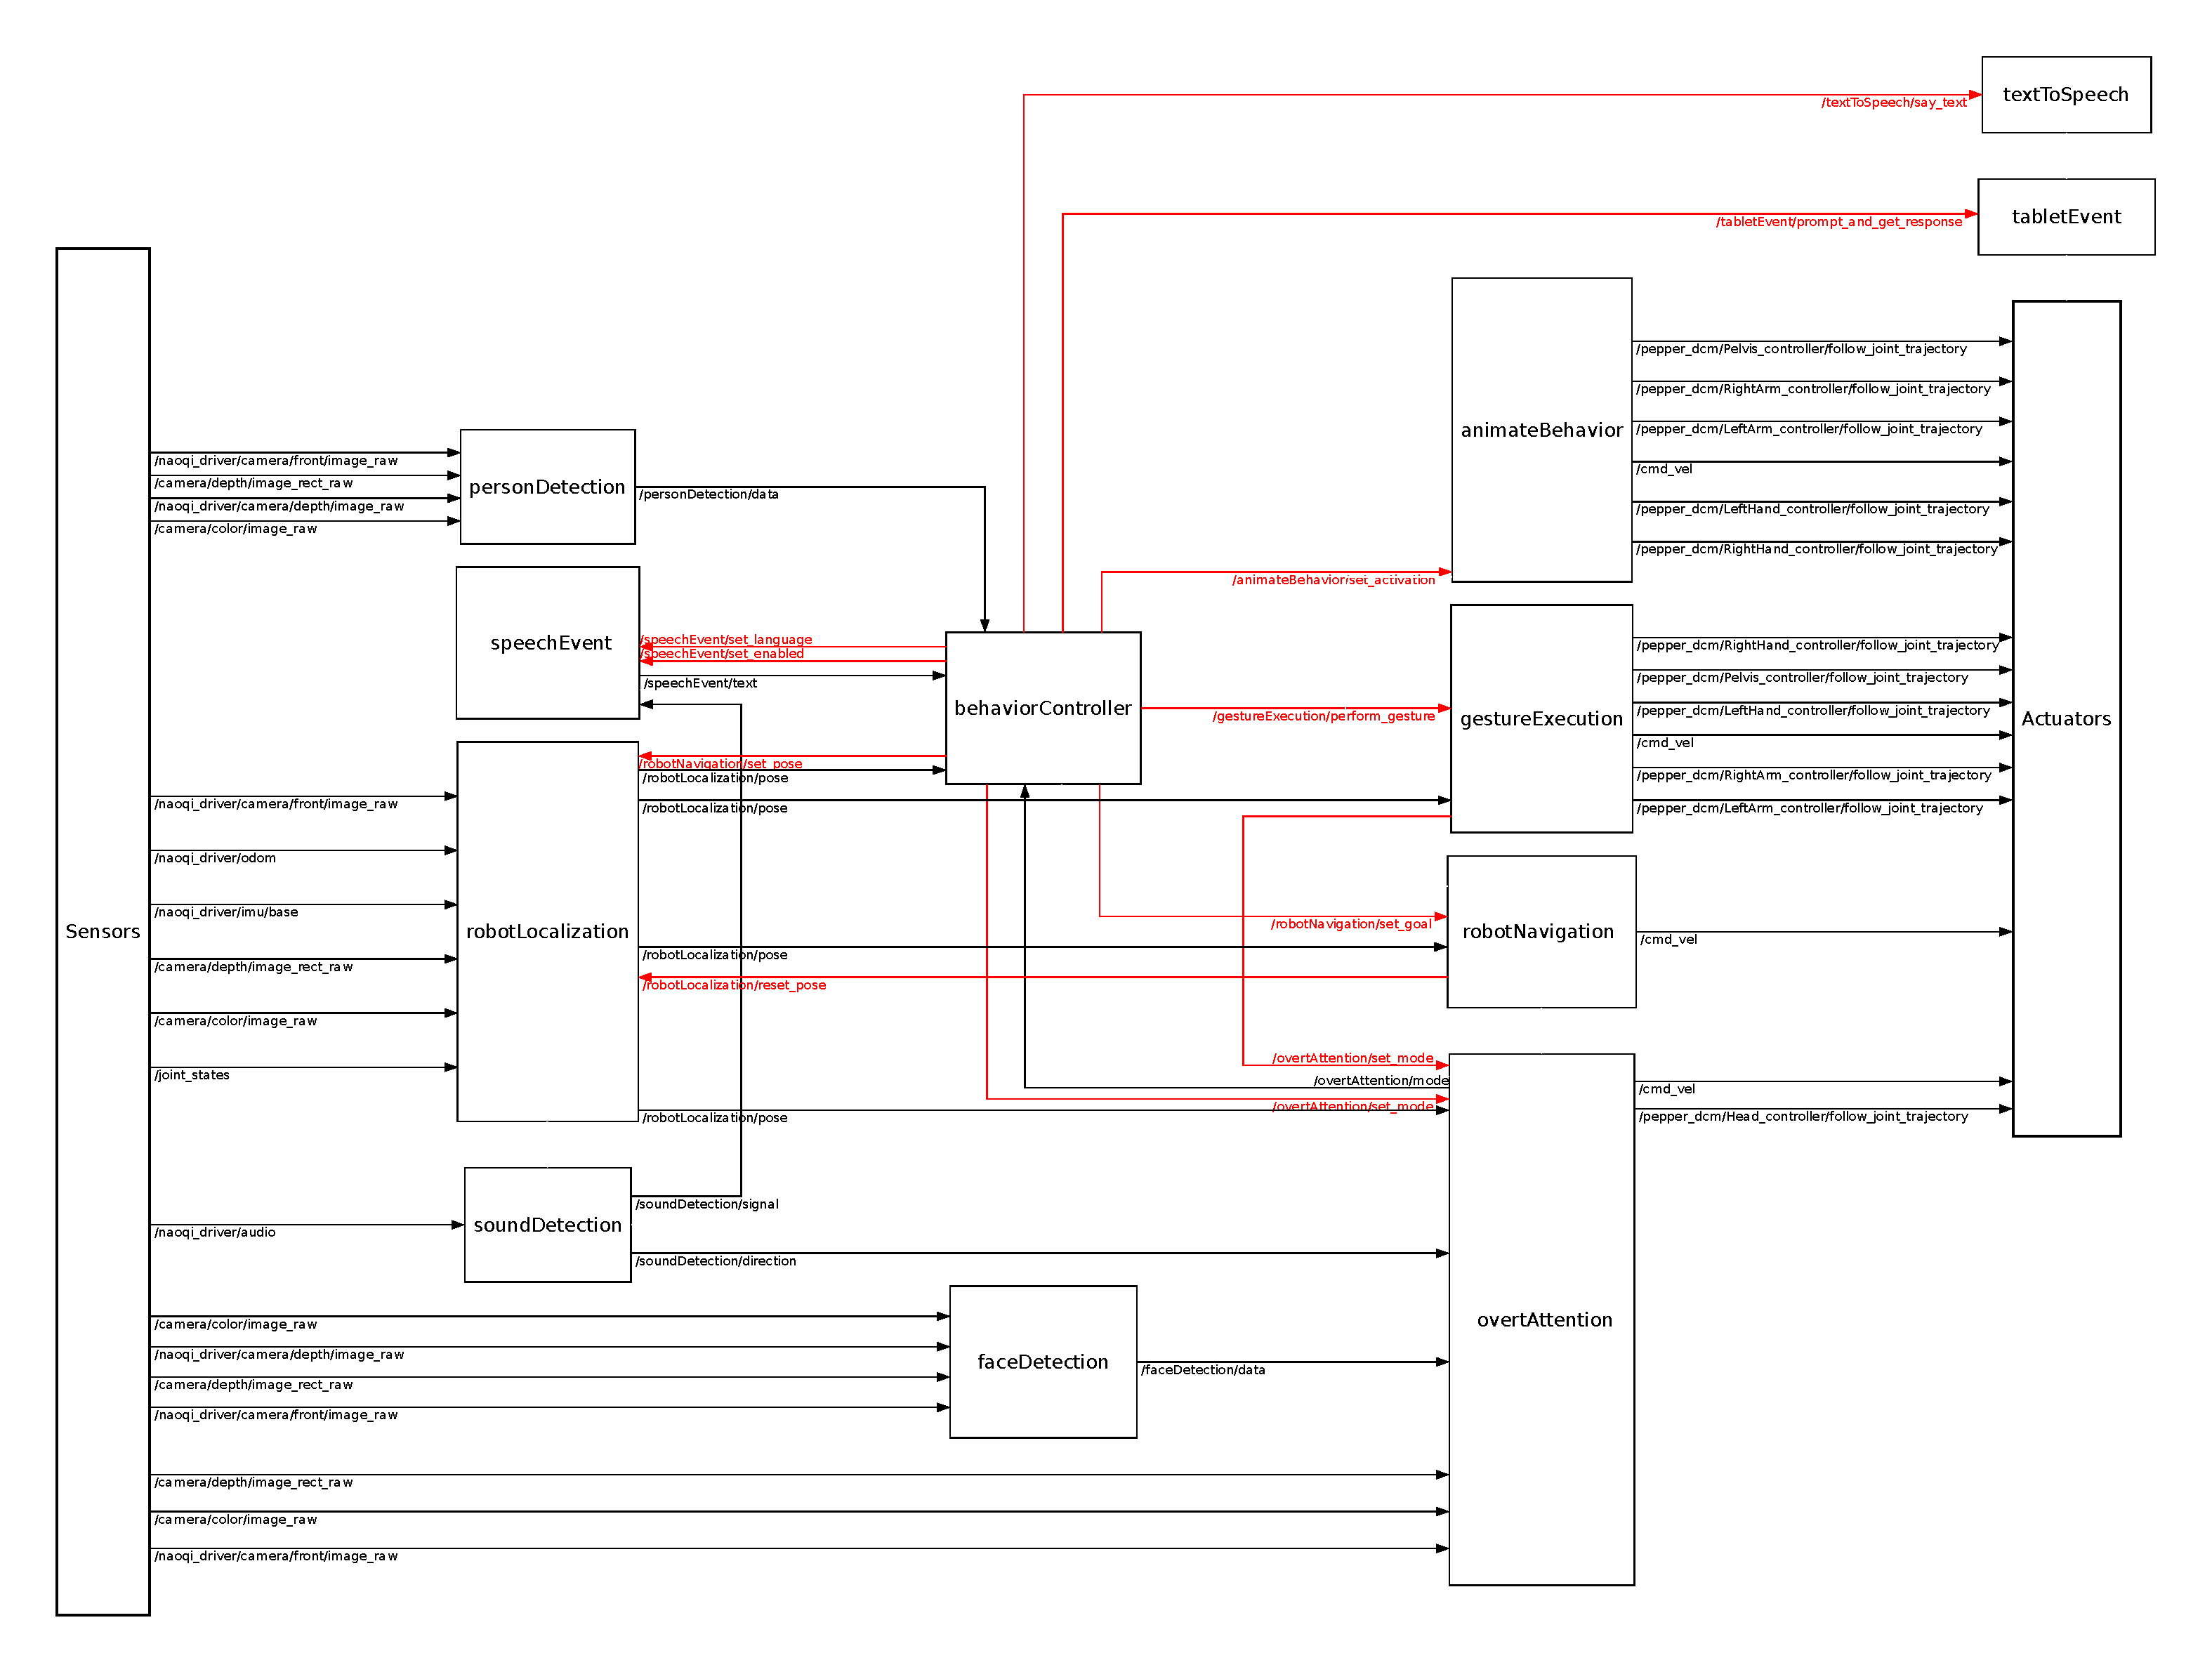
\includegraphics[width=165mm,angle=0]{System_Architecture_Nodes.pdf}
%\end{center}

\caption{The CSSR4Africa system architecture specified at the level of ROS nodes (thin border rectangles), ROS topics (black lines), ROS services (red lines), and sources \& sinks for sensor topics and actuator topics (thick border rectangles).}  
\label{fig:architecture2}       
\end{figure}

\clearpage

\newpage
\bibliographystyle{unsrt}
%================================================================
\bibliography{cognitive_systems.bib}                                     % REPLACE with correct filename
\addcontentsline{toc}{section}{References}



\pagebreak
\section*{Principal Contributors}
%===============================================================
\label{contributors}
\addcontentsline{toc}{section}{Principal Contributors}
The main authors of this deliverable are as follows (in alphabetical order).
\blank
~
\blank
Muhammed Danso, Carnegie Mellon University Africa.\\   
David Vernon, Carnegie Mellon University Africa.\\   
Yohannes Haile, Carnegie Mellon University Africa.\\

\newpage
\section*{Document History}
%================================================================
\addcontentsline{toc}{section}{Document History}
\label{document_history}

\begin{description}

\item [Version 1.0]~\\
First draft. \\
David Vernon. \\                          
24 January 2024.

\item [Version 1.1]~\\
Added a configuration file for {\small \verb+tabletEvent+}.\\
David Vernon. \\                          
25 January 2024.

\item [Version 1.2]~\\
Added key-value pair for {\small \verb+personDetection+} and {\small \verb+factDetection+} to specify the algorithm to be used.\\
David Vernon. \\                          
01  February 2024.

\item [Version 1.3]~\\
Updated topics for the  {\small \verb+animateBehavior+} and  {\small \verb+gestureExecution+}  nodes, replacing {\small \verb+command+}, with {\small \verb+follow_joint_trajectory+}. Updated topics for the {\small \verb+soundDetection+} node.\\
Removed  {\small \verb+/pepper/camera/stereo/image_raw+} topic for simulator in the  {\small \verb+faceDetection+},  {\small \verb+overtAttention+},  {\small \verb+personDetection+}, and  {\small \verb+robotLocalization+}    nodes.\\
Added {\footnotesize \verb+behaviorController+} to the list of nodes to which {\footnotesize \verb+robotLocalization+} publishes.\\
David Vernon. \\                          
09  May 2024.

\item [Version 1.4]~\\
Updated topics for the  {\small \verb+overtAttention+}  to include a topic on which the mode is published.\\
Muhammed Danso. \\                          
27 August 2024.


\item [Version 1.5]~\\
Changed  {\small \verb+scriptInterpreter+}  to {\small \verb+behaviorController+}.\\
Amended some of the Version 1.4 updates.\\
David Vernon. \\                          
28 August 2024.

\item [Version 1.6]~\\
Removed   {\small \verb+waypointNumber+}  and {\small \verb+waypointSelection+} keys  from  {\small \verb+robotNavigation+}. \\
Changed the specification of the pose in the {\small \verb+robotNavigation/set_goal+} service from using {\small \verb+geometry_msgs/Pose.msg+} with {\small \verb+<Point> <Quaternion>+}  to a custom message with  {\small \verb+<x> <y> <theta>+} .\\
Changed references to script language and script interpreter to robot mission language and robot mission interpreter.\\
David Vernon. \\                          
09 September 2024.

\item [Version 1.7]~\\
Updated scanning mode for the {\small \verb+overtAttention+} to prioritize detected faces when scanning the environment for general features.\\
Updated {\small \verb+gestureExecution+} to include head movement to complement pointing gestures. (with the help of Adedayo)\\
Updated  {\small \verb+faceDetection+} to remove eye detection and add mutual gaze detection. (with the help of Yohannes)\\
Updated Figure \ref{fig:architecture2} system architecture.
Muhammed Danso. \\                          
21 December 2024.

\item [Version 1.8]~\\
Removed {\small \verb+/naoqi_driver/camera/stereo/image_raw+ } from {\small \verb+overtAttention+}, {\small \verb+personDetection+}, and {\small \verb+robotLocalization+} .
Added {\small \verb+/camera/color/image_raw+ } and {\small \verb+/camera/depth/image_rect_raw+ }  to  {\small \verb+overtAttention+}, {\small \verb+personDetection+}, and {\small \verb+robotLocalization+} .\\ 
Changed option for selecting camera from {\small \verb+StereoCamera+}  to {\small \verb+RealSense+} in   {\small \verb+overtAttention+}, {\small \verb+personDetection+} and {\small \verb+robotLocalization+} . \\
Updated the GraphViz architecture diagram to reflect these changes.\\
David Vernon. \\                          
1 January 2025.

\item [Version 1.9]~\\
Changed the configuration file from \texttt{faceDetectionConfiguration.ini} to \\ \texttt{faceDetectionConfiguration.json}\\
Updated the face Detection Configuration file key-value pairs table. \\
Fixed error on the Topics Subscribed overAttention node. \\
Removed a statement in the Sound Detection regrading message type.\\
Fixed error on Topics Published on Person Detection.\\
Yohannes Haile. \\
16 January 2025.

\item [Version 1.10]~\\
Moved {\small \verb+behaviorController+ } to keep the ROS nodes in alphabetic order, and renamed the Section Robot Mission Interpreter to Behavior Controller.\\
David Vernon. \\                          
20 January 2025.

\item [Version 1.11]~\\
Changed Interaction Scenario Manager subsystem to Robot Mission Interpreter subsystem. \\
Changed Interaction Manager in Figure \ref{fig:architecture1} to Robot Mission Interpreter and added the Environment Knowledge Base.\\
Removed {\small \verb+knowledgeBase+ } node.\\
Added subsections on the  {\small \verb+CultureKnowledgeBase+} and {\small \verb+EnvironmentKnowledgeBase+} helper classes in Sections \ref{section:behavior_controller} and \ref{section:robot_navigation}, respectively.\\
David Vernon. \\                          
29 January 2025.

\item [Version 2.0]~\\
Revised the system architecture to limit the support for the simulator.  Simulator support will not be provided for  ROS nodes that have the option of using an external device such as the RealSense camera or a LiDAR, or that use the Pepper microphones, speakers, or the tablet PC, or are dependent on data produced by these nodes. Consequently, the only node that supports the simulator is Animate Behavior.
Since this is a major revision, the version number is advanced to 2.0.\\
David Vernon.\\
1 February 2025.

\item [Version 2.1]~\\
Fixed incorrect reference to {\small \verb+personDetection+} in documenting the topics to which the {\small \verb+robotNavigation+} node publishes.\\
David Vernon.\\
9 February 2025.

\item [Version 2.2]~\\
Updated the functional descriptions of   {\small \verb+soundDetection+} and  {\small \verb+speechEvent+}.  Updated the configuration file specification of  {\small \verb+speechEvent+} and the services it supports. \\
David Vernon.\\
26 March 2025.

\item [Version 2.3]~\\
Added an option to use compressed images for \texttt{faceDetection} and \texttt{personDetection}. \\
Added compressed image option in the configuration file table \texttt{faceDetection} and \\
\texttt{personDetection}.\\
Added topics of the compressed images for the topics Subscribed  for \texttt{faceDetection}.\\
Added topics of the compressed images for the topics Subscribed for \texttt{personDetection}.\\
Updated the person and face detection configuration file to camel case.\\
Added width and height as one component of the array of records.\\
\textcolor{blue}{Blue text} is used to mark addition of text or table entries and \textcolor{red}{red text} was used to mark deletion of
text or table entries will be changed to black in the next version.\\
Yohannes Haile.\\
31 March 2025.


\item [Version 2.4]~\\
Added a service  {\small \verb+/robotLocalization/set_pose+} and a call from  {\small \verb+behaviorController+}.\\
Changed behaviour to behavior globally. This mainly affects  {\small \verb+animateBehavior+}\\
Removed the red text in the previous version and changed the blue text to black.
David Vernon.\\
7 May 2025.

\item [Version 2.5]~\\
In the configuration file table {\small \verb+textToSpeechConfiguration.ini+}. Added three configurable components which are {\small \verb+ robot's Ip, port, and use_cuda.+} \\
Also added another service request {\small \verb+ string <language>+} to the service support table in 3.12.

Muhirwa Richard.\\
02 June 2025.

\item [Version 2.6]~\\
Update {\small \verb+speechEvent+} to publish ``Error: soundDetection is down'' when {\small \verb+soundDetection+} is unavailable \\
Open a graphical application that displays text transcriptions on the screen when {\small \verb+speechEvent+} is run in verbose mode \\
Add {\small \verb+confidence+}, {\small \verb+speechPausePeriod+} and {\small \verb+maxUtteranceLength+} configuration options to {\small \verb+speechEvent+}'s configuration file \\
Add support for the {\small \verb+/speechEvent/set_enabled+} ROS service to {\small \verb+speechEvent+} \\
Use an updated system architecture diagram to show the new {\small \verb+/speechEvent/set_enabled+} ROS service \\
Clifford Onyonka.\\
11 June 2025.


\end{description}

\end{document}











\newpage

\subsection{Knowledge Base}
%=================================================================================

\subsubsection*{ROS Node Name}
%----------------------------
 {\normalsize \verb+knowledgeBase+}   

\subsubsection*{Functional Specification}
%--------------------------------
This ROS node   provides a server for a culture knowledge ontology and a related knowledge base that, together, formalize the culturally sensitive knowledge that is documented in Deliverables D1.2 African Modes of Social Interaction and D1.3 Africa-centric Design Patterns.  It provides the basis for generating culturally sensitive actions by the robot when interacting with visitors in the use case demonstrations.   
  
The content and organization of the knowledge ontology and knowledge base has not yet been defined. This will be done in Task 5.4.1 and documented in Deliverable D5.4.1. 

The node can run in normal mode or verbose mode. In verbose mode, data that is published to topics is also printed to the terminal.

\subsubsection*{Configuration File}
%-----------------------------

The operation of the {\small \verb+knowledgeBase+} node is determined by the contents of a configuration file that  contain a list of key-value pairs as shown below.  

\noindent The configuration file is named {\small \verb+knowledgeBaseConfiguration.ini+}.

\begin{center}
\begin{tabularx}{\linewidth}{| l | l | X|}
\hline 
{\small Key }                               & {\small Values }                                                 &  {\small Effect}       \\
\hline
{\footnotesize \verb+knowledgeOntology+}  & {\footnotesize \verb+knowledgeOntology.dat+}     & {\small Specifies the filename of the file in which theknowledge ontology stored.} \\
\hline
{\footnotesize \verb+knowledgeBase+}  & {\footnotesize \verb+knowledgeBase.dat+}     & {\small Specifies the filename of the file in which the knowledge base stored.} \\
\hline
{\footnotesize \verb+verboseMode+}  & {\footnotesize \verb+true+, \verb+false+}     & {\small Specifies whether diagnostic data is to be printed to the terminal.} \\
\hline
\end{tabularx}
\end{center}

\subsubsection*{Input Data File}
%--------------------------
This node reads the knowledge ontology file and the knowledge base file specified in the configuration file.


\subsubsection*{Output Data File}
%----------------------------
This node does not write to an output data file.


\subsubsection*{Topics Subscribed}
%-----------------------------
This node  does not subscribe to any topics.

 

\subsubsection*{Topics Published}
%----------------------------
This node does not publish to any  topics.

\subsubsection*{Services Supported}
%---------------------------------------
This node  provides and advertizes a server for a service {\small \verb+/knowledgeBase/query+} to extract required knowledge from the knowledge base.    

The type of the variable that is passed as an argument to the service call  has not yet been defined. This will be done when the knowledge ontology and knowledge base has been specified  in Task 5.4.1 and when the specification of the robot mission interpreter in Task 5.4.3 is complete.
 
The type of the service call  return value has not yet been defined. Again, this will be done when the knowledge ontology and knowledge base has been defined  in Task 5.4.1 and when the specification of the robot mission interpreter in Task 5.4.3 is complete.

The service  is called by  the {\small \verb+behaviorController+} and {\small \verb+robotNavigation+} nodes.

The following summarizes the services supported.

\begin{center}
\begin{tabularx}{\linewidth}{| l | l | X|}
\hline 
{\small Service }                                                    & {\small Message Value}    &  {\small Effect}       \\
\hline
{\footnotesize \verb+/knowledgeBase/query+ }  & To be defined & {\small Extract required knowledge from the knowledge base} \\ 
\hline
\end{tabularx}
\end{center}

\subsubsection*{Services Called}
%---------------------------------------
This node does not call any services.




